\documentclass[12pt]{article}
%
\usepackage{abstract,amsmath,amssymb,latexsym}
\usepackage{enumitem,epsf}
\usepackage{fullpage,tikz,float}
\usepackage[numbers]{natbib}
\usepackage[pdftex,colorlinks]{hyperref}

% locally defined macros
\usepackage{macros}

%%%%%%%%%%%%%%%%%%%%%%%%%%%%%%%%%%%%%%%%%%%%%%%%%%%%%%%%%%%%%

% Use the following for revealing TODOs and appendices
% Options are: \draftfalse or \drafttrue
\newif\ifdraft
\draftfalse

%%%%%%%%%%%%%%%%%%%%%%%%%%%%%%%%%%%%%%%%%%%%%%%%%%%%%%%%%%%%%

\title{
 \begin{minipage}[c]{1.05\textwidth}
 	\centerline{Toward Deeper Understanding of Neural Networks:}
 	\centerline{The Power of Initialization and a Dual View on Expressivity}
 \end{minipage}
}

\author{
	\vspace{1cm}
  Amit Daniely\thanks{Email: amitdaniely@google.com} \and
  Roy Frostig\thanks{Email: rf@cs.stanford.edu. Work performed at Google.} \and
  Yoram Singer\thanks{Email: singer@google.com}
}

\begin{document}

\maketitle
\thispagestyle{empty}

%% \vspace{-4cm}
%% \vspace*{\fill} {
%% \renewcommand{\abstractnamefont}{\normalfont\large\bfseries}
%% \renewcommand{\abstracttextfont}{\normalfont\normalfont}
%% \renewcommand{\baselinestretch}{1.0}
\begin{abstract}
%% \vspace{-0.25cm}

\begin{abstract}
Language models (LMs), like other neural networks, often favor shortcut heuristics based on surface-level patterns.
Although LMs behave like n-gram models early in training, they must eventually learn hierarchical syntactic representations to correctly apply grammatical rules out-of-distribution (OOD).
In this work, we use case studies of English grammar to explore how complex, diverse training data drives models to generalize OOD. We construct a framework that unifies our understanding of random variation with training dynamics, rule selection with memorization, and data diversity with complexity. 
We show that these factors are nuanced, and that intermediate levels of diversity and complexity lead to inconsistent behavior across random seeds and to unstable training dynamics. 
Our findings emphasize the critical role of training data in shaping generalization patterns and illuminate how competing model strategies lead to inconsistent generalization outcomes across random seeds. Code is available at \url{https://github.com/sunnytqin/concept_comp.git}.

\end{abstract}

\end{abstract}
%% }
%% \vspace*{\fill}

\ifdraft
\newpage
\section{Flows for trees and uniform distributions}


ping

\textcolor{blue}{
\textbf{To-do list (sensitivity analysis):}
\begin{enumerate}
    \item Sensitivity analysis for regular trees and uniform distribution 
    \item Generalization for DAGs
    \item Generalization for non-uniform distributions
\end{enumerate}
}
\textcolor{orange}{
\textbf{To-do list (policy networks):}
\begin{enumerate}
    \item Anonymous
    \begin{enumerate}
        \item Balance is impossible for some pairs of pointed DAGs and reward functions
        \item Some characterization of rewards that are particularly hard to approximate
        \item Sequences, Multisets, Anonymous and non-anonymous graphs (directed and undirected) 
\item trade-off between invariances in the networks and built into the state graph    \end{enumerate}
    \item Non-anonymous
\end{enumerate}
    }

\textcolor{red}{
\textbf{To-do list (evaluation and diagnostic of GFLowNets):}
\begin{enumerate}
    \item Current evaluation protocols are crap (usually focus on covering modes rather than approximation). Doing the right thing is also computationally infeasible for larges state-spaces 
    \item Convergence diagnostic based on some estimate of $\delta$, leveraging our theorems in the first part of the paper
    \item some diagonose based on, e.g, the estimates we can get from $R$ based on the trajectory-balance loss (in equilibrium, should be path independent, i.e., a constant)
\end{enumerate}
}


\fi

\newpage
\thispagestyle{empty}

{\large
\topskip0pt
\vspace*{\fill}
\tableofcontents
\vspace*{\fill}
}

\newpage

\setcounter{page}{1}

\section{Introduction}
%
Neural network (NN) learning has underpinned state of the art empirical
results in numerous applied machine learning tasks (see for
instance~\cite{krizhevsky2012imagenet,lecun2015deep}). Nonetheless, neural
network learning remains rather poorly understood in several regards.
Notably, it remains unclear why training algorithms find good weights, how
learning is impacted by the network architecture and activations, what is
the role of random weight initialization, and how to choose a concrete
optimization procedure for a given architecture.

We start by analyzing the expressive power of NNs subsequent to the random
weight initialization. The motivation is the empirical success of training
algorithms despite inherent computational intractability, and the fact that
they optimize highly non-convex objectives with potentially many local minima.
Our key result shows that random initialization already positions learning
algorithms at a good starting point. We define an object termed a {\em
computation skeleton} that describes a distilled structure of feed-forward
networks. A skeleton induces a family of network architectures along with a
hypothesis class $\ch$ of functions obtained by certain non-linear
compositions according to the skeleton's structure.  We show that the
representation generated by random initialization is sufficiently rich to
approximately express the functions in $\ch$. Concretely, all functions in
$\ch$ can be approximated by tuning the weights of the last layer, which is
a convex optimization task.

In addition to explaining in part the success in finding good weights, our
study provides an appealing perspective on neural network learning.  We
establish a tight connection between network architectures and their dual
kernel spaces. This connection generalizes several previous constructions
(see Sec~\ref{sec:related}). As we demonstrate, our dual view gives rise to
design principles for NNs, supporting current practice and suggesting
new ideas. We outline below a few points.

\begin{itemize}

\item Duals of convolutional networks appear a more suitable fit for
	vision and acoustic tasks than those of fully connected networks.

\item Our framework surfaces a principled initialization scheme. It is
	very similar to common practice, but incorporates a small correction.

\item By modifying the activation functions, two consecutive fully connected
	layers can be replaced with one while preserving the network's dual kernel.

\item The ReLU activation, i.e. $x \mapsto \max(x,0)$, possesses favorable
	properties. Its dual kernel is expressive, and it can be well approximated by
	random initialization, even when the initialization's scale is moderately
	changed.

\item As the number of layers in a fully connected network becomes very
	large, its dual kernel converges to a degenerate form for any non-linear
	activation.

\item Our result suggests that optimizing the weights of the last layer can
	serve as a convex proxy for choosing among different architectures prior
	to training. This idea was advocated and tested empirically
	in~\cite{saxe2011random}.

\end{itemize}

\vspace{-5pt}
\section{Related Work}
\label{sec:related}
\vspace{-8pt}
\noindent\textbf{Self-Supervised Learning.} 
Recent SSL approaches have shown performance comparable to their supervised learning equivalents~\cite{caron2020unsupervised, caron2021emerging, chen2020simple, he2020momentum, grill2020bootstrap, zbontar2021barlow, bardes2021vicreg, chen2020improved}. In a nutshell, most of these methods use image augmentation techniques to generate correlated views (positives) from a sample, and then learn a model that is invariant to these augmentations by enforcing the network to output similar representations for the positives. Initially, contrastive learning, based on instance discrimination~\cite{wu2018unsupervised} using noise-contrastive estimation~\cite{gutmann2010noise, oord2018representation}, was a popular strategy~\cite{chen2020simple, he2020momentum}. However, this learning paradigm 
requires large batch sizes or memory banks. A few methods that use a negative-free cosine similarity loss~\cite{grill2020bootstrap, chen2021exploring} have addressed such issues.

Concurrently, clustering-based methods (SwAV~\cite{caron2020unsupervised}, DeepCluster v2~\cite{caron2020unsupervised, caron2018deep} and DINO~\cite{caron2021emerging}) have also been proposed. They do not operate on the features directly, and instead compare positives through a cross-entropy loss using cluster prototypes as a proxy. Redundancy reduction-based methods have also been popular\cite{ermolov2021whitening, zbontar2021barlow, bardes2021vicreg}. Among them, BarlowTwins \cite{zbontar2021barlow} considers an objective function measuring the cross-correlation matrix between the features, and VicReg\cite{bardes2021vicreg} uses a mix of variance, invariance and covariance
regularizations. Methods such as~\cite{dwibedi2021little} have explored the use of nearest-neighbour retrieval and divide and conquer~\cite{tian2021divide}. However, none of these works studied the ability of SSL methods to learn continually and adaptively.


\noindent\textbf{Continual Learning.} A plethora of methods have been developed to counteract catastrophic forgetting~\cite{kirkpatrick2017overcoming, Rusu16progressive, shin2017continual, Lopez-Paz17, Chaudhry19, serra2018overcoming, chaudhry2018riemannian, Aljundi17, Zenke17, buzzega2020dark, fini2020online, douillard2020podnet, wu2019large, castro2018end, rebuffi2017icarl, hou2019learning, prabhu2020gdumb, Li17learning, ostapenko2019learning, cha2021co2l, Robins95}. Following~\cite{de2019continual}, these works can be organized into three macro-categories: replay-based~\cite{ostapenko2019learning, Robins95, rebuffi2017icarl, buzzega2020dark, Chaudhry19, Lopez-Paz17}, regularization-based~\cite{fini2020online, Li17learning, shin2017continual, kirkpatrick2017overcoming, Zenke17, Aljundi17, castro2018end, douillard2020podnet, hou2019learning, chaudhry2018riemannian, wu2019large, cha2021co2l}, and parameter isolation
methods~\cite{Rusu16progressive, serra2018overcoming}. All these works evaluate the effectiveness of CL methods using a linear classifier learned
sequentially over time. However, this evaluation does not reflect an important aspect, \textit{i.e.}, the internal dynamics of the hidden representations. Moreover, most CL methods tend to rely on supervision in order to mitigate catastrophic forgetting. A few of them can be adapted for the unsupervised setting, although their effectiveness is greatly reduced (see discussion in Sec.~\ref{sec:cassowary}, Sec.~\ref{sec:experiments} and the supplementary material). 

Works such as~\cite{rao2019continual, achille2018life, smith2019unsupervised} laid the foundations of unsupervised CL, but their studies are severely limited to digit-like datasets, \emph{e.g.}, MNIST and Omniglot, and the proposed methods are unfit for large-scale scenarios. Recently, \cite{gallardo2021self, caccia2021special} explored self-supervised pretraining for supervised continual learning with online and few-shot tasks, and \cite{cha2021co2l} presented a supervised contrastive CL approach. Two concurrent works~\cite{lin2021continual, madaan2021rethinking} have also attempted to address CSSL recently. The former~\cite{lin2021continual} extends~\cite{cha2021co2l} to the unsupervised setting, but is specifically designed for contrastive SSL, such as~\cite{chen2020simple,he2020momentum}, and lacks generalizability to other popular SSL paradigms. The latter~\cite{madaan2021rethinking} is also limited as it only shows small-scale experiments in the class-incremental setting and considers just two SSL methods. In contrast, we present a general framework for CSSL with superior performance, conduct large-scale experiments on three challenging settings, thereby presenting a deeper analysis of CSSL.
\section{Setting}

\paragraph{Notation.} We denote
%% scalars by lowercase and uppercase letters and (e.g., $x, X$),
vectors by bold-face letters (e.g.\ $\x$), and
matrices by upper case Greek letters (e.g.\ $\Sigma$). The $2$-norm of $\x
\in \reals^d$ is denoted by $\|\x\|$. For functions $\sigma:\reals\to\reals$
we let
$$
\|\sigma\| \textstyle
	:=\sqrt{\E_{X\sim\cn(0,1)}\sigma^2(X)}
	\; = \sqrt{\frac{1}{\sqrt{2\pi}}
		\int_{-\infty}^\infty \sigma^2(x)e^{-\frac{x^2}{2}}dx} \,.
$$
%
Let $G=(V,E)$ be a directed acyclic graph. The set of neighbors incoming to
a vertex $v$ is denoted $\IN(v):=\{u\in V\mid uv\in E\}$.
%% The $d$ dimensional vector space of the reals is denoted by
%% $\reals^d$.
The $d-1$ dimensional sphere is denoted $\sphere^{d-1} =
\{\x\in\reals^d \mid \|\x\|=1\}$. We provide a brief overview of
reproducing kernel Hilbert spaces in the sequel and merely introduce
notation here. In a Hilbert space $\ch$, we use a slightly
non-standard notation $\ch^B$ for the ball of radius $B$, $\{\x \in
\ch \mid \|\x\|_\ch \leq B\}$. We use $[x]_+$ to denote $\max(x,0)$
and $\ind[b]$ to denote the indicator function of a binary variable
$b$.

\paragraph{Input space.} Throughout the paper we assume that each example is
a sequence of $n$ elements, each of which is represented as a unit vector. 
Namely, we fix $n$ and take the input space to be
	$\cx=\cx_{n,d}=\left(\sphere^{d-1}\right)^n$.
Each input example is denoted,
\begin{align} \label{eq:coordinates}
	\x=(\x^1,\ldots,\x^n), ~\textwhere \x^i\in \sphere^{d-1} \,.
\end{align}
%
We refer to each vector $\x^i$ as the input's $i$th {\em
  coordinate}, and use $x^i_{j}$ to denote it $j$th scalar
entry. Though this notation is slightly non-standard, it unifies 
input types seen in various domains. For example,
binary features can be encoded by taking $d=1$, in which case
$\cx=\{\pm 1\}^n$. Meanwhile, images and audio signals are often
represented as bounded and continuous numerical values---we can assume
in full generality that these values lie in $[-1,1]$. To match the setup
above, we embed $[-1,1]$ into the circle $\sphere^1$, e.g.\ via the map $x
\mapsto \left(\sin\left(\frac{\pi x}{2}\right), \cos\left(\frac{\pi
  x}{2}\right)\right)$. When each coordinate is categorical---taking
one of $d$ values---we can represent category $j\in[d]$ by the unit
vector $\mathbf e_j\in\sphere^{d-1}$. When $d$ may be very large or
the basic units exhibits some structure, such as when the input is a sequence
of words, a more concise encoding may be
useful, e.g.\ as unit vectors in a low dimension space $\sphere^{d'}$
where $d'\ll d$ (see for
instance~\citet{mikolov2013distributed,levy2014neural}).

\paragraph{Supervised learning.} The goal in supervised learning is to
devise a mapping from the input space $\cx$ to an output space $\cy$ based on a sample
$S=\{(\x_1,y_1),\ldots,(\x_m,y_m)\}$, where $(\x_i,y_i)\in\cx\times\cy$, 
drawn i.i.d.\ from a distribution $\cd$ over $\cx\times\cy$.
%
A supervised learning problem is further specified by an output length $k$ and a loss function
$\ell : \reals^k \times \cy \to [0,\infty)$, and the goal is to find a
predictor $h:\cx\to\reals^k$ whose loss,
$\cl_{\cd}(h) := \E_{(\x,y)\sim\cd} \ell(h(\x),y)$, is small.
%
The {\em empirical} loss $\cl_{S}(h):= \frac 1 m \sum_{i=1}^m
\ell(h(\x_i),y_i)$ is commonly used as a proxy for the loss
$\cl_{\cd}$.
%
Regression problems correspond to $\cy=\reals$ and, for
instance, the squared loss $\ell(\hat y,y)=(\hat y -y)^2$.
%
Binary classification is captured by $\cy=\{\pm 1\}$ and, say, the
zero-one loss $\ell(\hat y,y)= \ind[\hat y y \leq 0]$ or the hinge
loss $\ell(\hat y,y)=[1-\hat y y]_+$, with standard extensions to the
multiclass case.
A loss $\ell$ is $L$-Lipschitz if $|\ell(y_1,y) - \ell(y_2,y) | \leq L
|y_1 - y_2|$ for all $y_1,y_2 \in \reals^k$, $y \in \cy$, and it is
convex if $\ell(\cdot,y)$ is convex for every $y\in\cy$.
%% Moreover, $\ell$ is
%% $L$-Lipschitz if $\ell(\cdot,y)$ is $L$-Lipschitz for every $y\in\cy$.

\paragraph{Neural network learning.} We define a {\em neural network} $\cn$
to be a vertices weighted directed acyclic graph (DAG) whose nodes are denoted $V(\cn)$ and edges
$E(\cn)$. The weight function will be denoted by $\delta:V(\cn)\to [0,\infty)$, and its sole role would be to dictate the distribution of the initial weights (see definition \ref{def:rand_weights}).
Each of its internal units, i.e.\ nodes with both incoming and
outgoing edges, is associated with an {\em activation} function
$\sigma_v:\reals\to\reals$. In this paper's context, an activation can
be any function that is square integrable with respect to the Gaussian
measure on $\reals$. We say that $\sigma$ is {\em normalized} if
$\|\sigma\|=1$. The set of nodes having only incoming edges are called the
output nodes.
%
To match the setup of a supervised learning problem, a network $\cn$ has
$nd$ input nodes and $k$ output nodes, denoted $o_1,\ldots,o_k$. A
network $\cn$ together with a weight vector $\w=\{w_{uv} \mid uv\in E\}$ defines a
predictor $h_{\cn,\w}:\cx\to\reals^k$ whose prediction
is given by ``propagating'' $\x$ forward through the network.
Formally, we define $h_{v,\w}(\cdot)$ to be the output of the subgraph
of the node $v$ as follows: for an input node $v$, $h_{v,\w}$ outputs the corresponding coordinate in $\x$, and
for all other nodes, we define $h_{v,\w}$ recursively as
$$h_{v,\w}(\x) = \sigma_v\left(\textstyle
	\sum_{u\in \IN(v)}\, w_{uv}\,h_{u,\w}(\x)\right)\,.$$
Finally, we let $h_{\cn,\w}(\x)=(h_{o_1,\w}(\x),\ldots,h_{o_k,\w}(\x))$.
We also refer to internal nodes as {\em hidden units}. The {\em output
layer} of $\cn$ is the sub-network consisting of all output neurons of $\cn$
along with their incoming edges. The {\em representation} induced by a network
$\cn$ is the network $\netrep(\cn)$ obtained from $\cn$ by removing the output
layer. The {\em representation} function induced by the weights $\w$ is
$\rep_{\cn,\w}:=h_{\netrep(\cn),\w}.$
Given a sample $S$, a learning algorithm searches
for weights $\w$ having small empirical loss
$\cl_S(\w)=\frac{1}{m}\sum_{i=1}^m \ell(h_{\cn,\w}(\x_i),y_i)$. A popular
approach is to randomly initialize the weights and then use a variant
of the stochastic gradient method to improve these weights in the
direction of lower empirical loss.

\paragraph{Kernel learning.} A function $\kappa:\cx\times \cx\to \reals$ is
a {\em reproducing kernel}, or simply a kernel, if for every
$\x_1,\ldots,\x_r\in\cx$, the $r \by r$ matrix $\Gamma_{i,j} = \{\kappa(\x_i,\x_j)\}$
is positive semi-definite. Each kernel induces a Hilbert space
$\ch_{\kappa}$ of functions from $\cx$ to $\reals$ with a corresponding norm
$\|\cdot\|_{\ch_\kappa}$. A kernel and its corresponding space are {\em
normalized} if $\forall \x\in\cx,\;\kappa(\x,\x)=1$. Given a convex loss
function $\ell$, %$:\reals^k\times \cy\to [0,\infty)$,
a sample $S$, and a kernel
$\kappa$, a kernel learning algorithm finds a function
$f=(f_1,\ldots,f_k)\in\ch^k_{\kappa}$ whose empirical loss,
$\cl_S(f)=\frac{1}{m}\sum_i \ell(f(\x_i),y_i)$, is minimal among all
functions with $\sum_{i}\|f_i\|_\kappa^2 \le R^2$ for some $R>0$.
Alternatively, kernel algorithms minimize the {\em regularized loss},
$$\cl^R_S(f)=\frac{1}{m}\sum_{i=1}^m \ell(f(\x_i),y_i) +
\frac{1}{R^2}\sum_{i=1}^k\|f_i\|^2_{\kappa} \,, $$
a convex objective that often can be efficiently minimized.

\section{Computation skeletons}
%
In this section we define a simple structure which we term a computation
skeleton. The purpose of a computational skeleton is to compactly describe
a feed-forward computation from an input to an output. A single skeleton encompasses a family of neural networks
that share the same skeletal structure. Likewise, it defines a
corresponding kernel space.
%
\begin{definition} A {\em computation skeleton} $\cs$ is a DAG whose
non-input nodes are labeled by activations.
\end{definition}
%
Though the formal definition of neural networks and skeletons appear
identical, we make a conceptual distinction between them as their role in
our analysis is rather different. Accompanied by a set of weights, a neural
network describes a concrete function, whereas the skeleton stands for a
topology common to several networks as well as for a kernel.
To further underscore the differences we note that skeletons are naturally more compact than networks. In particular, all examples of
skeletons in this paper are {\em irreducible}, meaning that for
each two nodes $v,u\in{}V(\cs)$, $\IN(v)\neq\IN(u)$.
We further restrict our attention
to skeletons with a single output node, showing later that single-output
skeletons can capture supervised problems with outputs in $\reals^k$. We
denote by $|\cs|$ the number of non-input nodes of $\cs$.

\begin{figure}[t]
\begin{center}
\begin{tikzpicture}
\foreach \i in {1,...,4}
{
	\draw (\i -7,0) rectangle (\i-7+0.5,0.5);
	\draw [->] (\i-7 +0.25  ,0.5) -- (-4.25 ,1);
}
\draw (-4.5,1) rectangle (-4,1.5);
\draw [->] (-4.25 ,1.5) -- (-4.25 ,2);
\node[text width=3cm] at (-2.85,-0.25) {$\cs_1$};
\foreach \i in {1,...,4}
{
	\draw (\i -1,0) rectangle (\i-1+0.5,0.5);
}
\foreach \i in {1,...,3}
{
	\draw (\i-1 + 0.5 ,1) rectangle (\i-1+1,1.5);
	\draw [->] (\i-1 +0.25  ,0.5) -- (\i-1 + 0.75 ,1);
	\draw [->] (\i-1 +1.25  ,0.5) -- (\i-1 + 0.75 ,1);
	\draw [->] (\i-1 + 0.75 ,1.5) -- (1.75 ,2);
}
\draw (1.5 ,2) rectangle (2,2.5);
\draw [->] (1.75 ,2.5) -- (1.75 ,3);
\node[text width=3cm] at (3.15,-0.25) {$\cs_2$};
\end{tikzpicture}
%
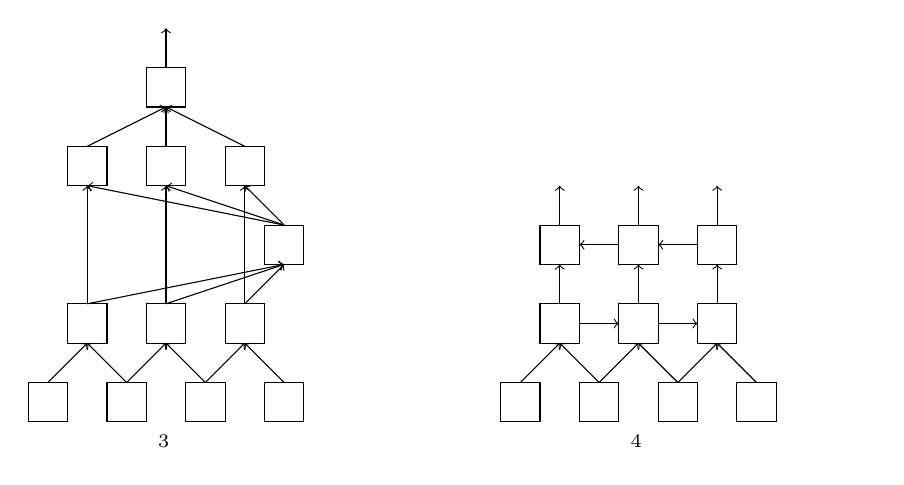
\begin{tikzpicture}
\foreach \i in {1,...,4}
{
	\draw (\i -7,0) rectangle (\i-7+0.5,0.5);
}
\foreach \i in {1,...,3}
{
	\draw (\i-7 + 0.5 ,1) rectangle (\i-7+1,1.5);
	\draw [->] (\i-7 +0.25  ,0.5) -- (\i-7 + 0.75 ,1);
	\draw [->] (\i-7 +1.25  ,0.5) -- (\i-7 + 0.75 ,1);
	\draw [->] (\i-7 + 0.75 ,1.5) -- (-2.75 ,2);
}
\draw (-3 ,2) rectangle (-2.5,2.5);
\foreach \i in {1,...,3}
{
	\draw (\i-7 + 0.5 ,3) rectangle (\i-7+1,3.5);
	\draw [->] (\i-7 +0.75, 1.5) -- (\i-7 +0.75,3);
	\draw [->] (-2.75, 2.5) -- (\i-7 +0.75,3);
	\draw [->] (\i-7 + 0.75 ,3.5) -- (-4.25 ,4);
}
\draw (-4.5 ,4) rectangle (-4,4.5);
\draw [->] (-4.25 ,4.5) -- (-4.25 ,5);
\node[text width=3cm] at (-2.85,-0.25) {$\cs_3$};
\foreach \i in {1,...,4}
{
	\draw (\i -1,0) rectangle (\i-1+0.5,0.5);
}
\foreach \i in {1,...,3}
{
	\draw (\i-1 + 0.5 ,1) rectangle (\i-1+1,1.5);
	\draw [->] (\i-1 +0.25  ,0.5) -- (\i-1 + 0.75 ,1);
	\draw [->] (\i-1 +1.25  ,0.5) -- (\i-1 + 0.75 ,1);
	\draw [->] (\i-1 + 0.75 ,1.5) -- (\i-1 + 0.75 ,2);
}
\draw [->] (1 ,1.25) -- (1.5 ,1.25);
\draw [->] (2 ,1.25) -- (2.5 ,1.25);
\foreach \i in {1,...,3}
{
	\draw (\i-1 + 0.5 ,2) rectangle (\i-1+1,2.5);
	\draw [->] (\i-1 + 0.75 ,2.5) -- (\i-1 + 0.75 ,3);
}
\draw [->] (1.5 ,2.25) -- (1 ,2.25);
\draw [->] (2.5 ,2.25) -- (2 ,2.25);
\node[text width=3cm] at (3.15,-0.25) {$\cs_4$};
\end{tikzpicture}
\caption{Examples of computation skeletons.\label{fig:cs_examples}}
\end{center}
\end{figure}

Figure \ref{fig:cs_examples} shows four example skeletons, omitting
the designation of the activation functions. The skeleton
$\cs_1$ is rather basic as it aggregates all the inputs in a single
step. Such topology can be useful in the absence of any prior
knowledge of how the output label may be computed from an input example, and
it is commonly used in natural language processing where the input is
represented as a bag-of-words~\cite{harris1954distributional}. The only structure in $\cs_1$
is a single {\em fully connected} layer:
\begin{terminology}[Fully connected layer of a skeleton]
%
An induced subgraph of a skeleton with $r+1$ nodes, $u_1,\ldots,u_r,v$, is
called a {\em fully connected layer} if its edges are
$u_1v,\ldots,u_rv$.
%
\end{terminology}
The skeleton $\cs_2$ is slightly more involved: it first processes
consecutive (overlapping) parts of the input, and the next layer
aggregates the partial results. Altogether, it corresponds to networks
with a single one-dimensional convolutional layer, followed by a fully
connected layer. The two-dimensional (and deeper) counterparts of such skeletons
correspond to networks that are common in visual object recognition.
\begin{terminology}[Convolution layer of a skeleton]
%
Let $s,w,q$ be positive integers and denote $n=s(q-1)+w$. A subgraph
of a skeleton is a one dimensional {\em convolution layer} of width $w$ and stride $s$
if it has $n+q$ nodes, $u_1,\ldots,u_{n}, v_1,\ldots,v_q$, and $q w$ edges,
$u_{s(i-1)+j}\,v_{i}$, for $1\le i\le q,1\le j\le w$.
%
\end{terminology}
%% The skeleton $\cs_3$ is a somewhat more sophisticated version of $\cs_2$, in
%% which after the local computations, a global computation is carried out
%% through a single aggregation node. The local computations are then
%% reassessed and finally aggregated again. The last skeleton, $\cs_4$, can be
%% useful for learning sequence-to-sequence mappings and similar skeletons
%% often used in translation, speech recognition, and OCR tasks.
The skeleton $\cs_3$ is a somewhat more sophisticated version of $\cs_2$: the local computations are first aggregated, then reconsidered with the aggregate, and finally aggregated again.
%
The last skeleton, $\cs_4$, corresponds to the networks that arise in
learning sequence-to-sequence mappings as used in translation, speech
recognition, and OCR tasks (see for example~\citet{sutskever2014sequence}).

\subsection{From computation skeletons to neural networks}
%
%% We are now ready to describe how a skeleton when accompanied with a
The following definition shows how a skeleton, accompanied with a
replication parameter $r\ge 1$ and a number of output nodes $k$,
induces a neural network architecture. Recall that inputs are ordered
sets of vectors in $\sphere^{d-1}$.
%% For brevity, we omit $d$ from the
%% notation introduced in the following definition.
%
\begin{definition}[Realization of a skeleton]
%
Let $\cs$ be a computation skeleton and consider input coordinates in
$\sphere^{d-1}$ as in \eqref{eq:coordinates}. For $r, k \ge 1$ we
define the following neural network $\cn=\cn(\cs,r,k)$.
%
For each input node in $\cs$, $\cn$ has $d$ corresponding input
neurons with weight $1/d$. For each internal node $v\in \cs$ labeled by an activation
$\sigma$, $\cn$ has $r$ neurons $v^1,\ldots,v^r$, each with an
activation $\sigma$ and weight $1/r$. In addition, $\cn$ has $k$ output neurons
$o_1,\ldots,o_k$ with the identity activation $\sigma(x)=x$ and weight $1$.
%
There is an edge $v^iu^j\in E(\cn)$ whenever $uv\in
E(\cs)$.  For every output node $v$ in $\cs$, each neuron $v^j$ is
connected to all output neurons $o_1,\ldots,o_k$. We term $\cn$ the
{\em $(r,k)$-fold realization} of $\cs$. We also define the {\em $r$-fold realization} of $\cs$ as\footnote{Note that for every $k$,
$\netrep\left(\cn(\cs,r,1)\right)=\netrep\left(\cn(\cs,r,k)\right)$.} $\cn(\cs,r)= \netrep\left(\cn(\cs,r,1)\right)$.
%
\end{definition}

%
\noindent
Note that the notion of the replication parameter $r$ corresponds, in
the terminology of convolutional networks, to the number of
channels taken in a convolutional layer and to the number of hidden units
taken in a fully-connected layer.
%% We would like to note that the architectures obtained by realizations of
%% skeletons include naturally many of the standard architectures employed in
%% practice such as fully connected layers, in which $r$ corresponds to the
%% number of hidden neurons, and convolutional layers, in which $r$ corresponds
%% to the number of channels.

Figure~\ref{fig:ct_to_nn} illustrates a $(5,4)$- and $5$-realizations
of a skeleton with coordinate dimension $d=2$.  The
$(5,4)$-realization is a network with a single (one dimensional)
convolutional layer having $5$ channels, stride of $2$, and width of
$4$, followed by three fully-connected layers. The global replication
parameter $r$ in a realization is used for brevity; it is
straightforward to extend results when the different nodes in $\cs$
are each replicated to a different extent.

%% We would also like to note that
%% for brevity, we use same replication parameter $r$ for all nodes. It is
%% straightforward to extend the definition and the results presented
%% henceforth to the case when different nodes in $\cs$ are associated with
%% different replication values.

\begin{figure}[t]
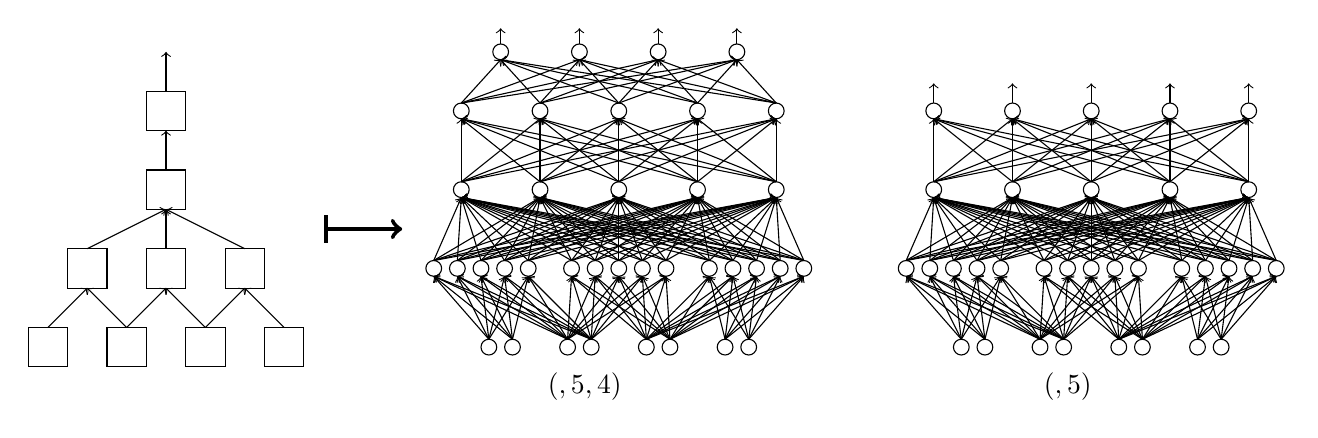
\begin{tikzpicture}
\foreach \i in {1,...,4}
{
	\draw (\i -1,0) rectangle (\i-1+0.5,0.5);
}
\foreach \i in {1,...,3}
{
	\draw (\i-1 + 0.5 ,1) rectangle (\i-1+1,1.5);
	\draw [->] (\i-1 +0.25  ,0.5) -- (\i-1 + 0.75 ,1);
	\draw [->] (\i-1 +1.25  ,0.5) -- (\i-1 + 0.75 ,1);
	\draw [->] (\i-1 + 0.75 ,1.5) -- (1.75 ,2);
}
\draw (1.5 ,2) rectangle (2,2.5);
\draw [->] (1.75 ,2.5) -- (1.75 ,3);
\draw (1.5 ,3) rectangle (2,3.5);
\draw [->] (1.75 ,3.5) -- (1.75 ,4);
\node[text width=3cm] at (3.15,-0.25) {$\cs$};
\draw [ultra thick, |->] (3.75,1.75) -- (4.75,1.75);
\foreach \i in {1,...,4}
{
	\draw (4.85+\i,0.25) circle [radius=0.1];
	\draw (5.15+\i,0.25) circle [radius=0.1];
}
\foreach \i in {-1,...,1}
{
	\foreach \j in {-2,...,2}
	{
		\draw (7.5+1.75*\i + 0.3*\j,1.25) circle [radius=0.1];
		\draw [->] (6.85+\i,0.35) -- (7.5+1.75*\i + 0.3*\j,1.15);
		\draw [->] (7.15+\i,0.35) -- (7.5+1.75*\i + 0.3*\j,1.15);

		\draw [->] (7.85+\i,0.35) -- (7.5+1.75*\i + 0.3*\j,1.15);
		\draw [->] (8.15+\i,0.35) -- (7.5+1.75*\i + 0.3*\j,1.15);
		\foreach \k in {-2,...,2}
		{
			\draw [->] (7.5+1.75*\i + 0.3*\j,1.35) -- (7.5+\k,2.15);
		}
	}
}
\foreach \j in {-2,...,2}
{
	\draw (7.5+\j,2.25) circle [radius=0.1];
	\foreach \k in {-2,...,2}
	{
		\draw[->] (7.5+\j,2.35) -- (7.5+\k,3.15);
	}
}
\foreach \j in {-2,...,2}
{
	\draw (7.5+\j,3.25) circle [radius=0.1];
	\draw[->] (7.5+\j,3.35) -- (6,3.9);
	\draw[->] (7.5+\j,3.35) -- (7,3.9);
	\draw[->] (7.5+\j,3.35) -- (8,3.9);
	\draw[->] (7.5+\j,3.35) -- (9,3.9);
}
\draw (6,4) circle [radius=0.1];
\draw (7,4) circle [radius=0.1];
\draw (8,4) circle [radius=0.1];
\draw (9,4) circle [radius=0.1];
\draw[->] (6,4.1) -- (6,4.3);
\draw[->] (7,4.1) -- (7,4.3);
\draw[->] (8,4.1) -- (8,4.3);
\draw[->] (9,4.1) -- (9,4.3);
\node[text width=3cm] at (8.1,-0.25) {$\cn(\cs,5,4)$};
\foreach \i in {1,...,4}
{
	\draw (10.85+\i,0.25) circle [radius=0.1];
	\draw (11.15+\i,0.25) circle [radius=0.1];
}
\foreach \i in {-1,...,1}
{
	\foreach \j in {-2,...,2}
	{
		\draw (6+7.5+1.75*\i + 0.3*\j,1.25) circle [radius=0.1];
		\draw [->] (6+6.85+\i,0.35) -- (6+7.5+1.75*\i + 0.3*\j,1.15);
		\draw [->] (6+7.15+\i,0.35) -- (6+7.5+1.75*\i + 0.3*\j,1.15);

		\draw [->] (6+7.85+\i,0.35) -- (6+7.5+1.75*\i + 0.3*\j,1.15);
		\draw [->] (6+8.15+\i,0.35) -- (6+7.5+1.75*\i + 0.3*\j,1.15);
		\foreach \k in {-2,...,2}
		{
			\draw [->] (6+7.5+1.75*\i + 0.3*\j,1.35) -- (6+7.5+\k,2.15);
		}
	}
}
\foreach \j in {-2,...,2}
{
	\draw (6+7.5+\j,2.25) circle [radius=0.1];
	\foreach \k in {-2,...,2}
	{
		\draw[->] (6+7.5+\j,2.35) -- (6+7.5+\k,3.15);
	}
}
\foreach \j in {-2,...,2}
{
	\draw (6+7.5+\j,3.25) circle [radius=0.1];
	\draw[->] (6+7.5+\j,3.35) -- (6+7.5+\j,3.6);
}
\node[text width=3cm] at (6+8.4,-0.25) {$\cn(\cs,5)$};
\end{tikzpicture}
\caption{A $(5,4)$-fold and $5$-fold realizations of the computation
skeleton $\cs$ with $d=2$.\label{fig:ct_to_nn}}
\end{figure}

We next define a scheme for random initialization of the weights of a neural
network, that is similar to what is often done in practice. We employ the definition throughout the paper whenever we refer to
random weights.
%
\begin{definition}[Random weights]\label{def:rand_weights}
%
A {\em random initialization} of a neural network $\cn$ is a
multivariate Gaussian $\w=(w_{uv})_{uv\in E(\cn)}$ such that each weight
$w_{uv}$ is sampled independently from a normal distribution with mean $0$
and variance\footnote{For $U\subset V(\cn)$ we denote $\delta(U) = \sum_{u\in U}\delta(u)$.} ${d\delta(u)}/{\delta(\IN(v))}$ if $u$ is an input neuron and ${\delta(u)}/{\left(\|\sigma_{u}\|^2\,\delta(\IN(v))\right)}$ otherwise.
%
\end{definition}
%
%% In practice, weights are often sampled independently from
%% normal distributions with variance proportional to ${1}/{|\IN(v)|}$.
%% We would like to note that in many architectures, such as convolutional nets,
\noindent
Architectures such as convolutional nets have weights that are shared
across different edges.
% (i.e.\ the same weight is associated with different edges)
Again, it is straightforward to extend our results to these cases and for
simplicity we assume no explicit weight sharing.

\subsection{From computation skeletons to reproducing kernels}
%
In addition to networks' architectures, a computation skeleton $\cs$ also
defines a normalized kernel $\kappa_\cs:\cx\times\cx\to[-1,1]$ and a
corresponding norm $\|\cdot \|_{\cs}$ on functions $f:\cx\to\reals$. This
norm has the property that $\|f\|_{\cs}$ is small if and only if $f$ can be
obtained by certain simple compositions of functions according to the
structure of $\cs$. To define the kernel,
we introduce a {\em dual activation} and {\em dual kernel}. For
$\rho\in[-1,1]$, we denote by $\gaussian_\rho$ the multivariate Gaussian
distribution on $\reals^2$ with mean $0$ and covariance matrix
$\left( \begin{smallmatrix} 1 & \rho \\ \rho & 1 \end{smallmatrix} \right)$.
%% whose diagonal elements are $1$ and off-diagonal elements are $\rho$.
%% \iffalse
%% $\begin{pmatrix} 1 & \rho \\ \rho & 1 \end{pmatrix}$.
%% \fi
%

\begin{definition}[Dual activation and kernel]\label{def:dual_act}
%
The {\em dual activation} of an activation $\sigma$ is the function
$\hat{\sigma}:[-1,1]\to\reals$ defined as
$$
\hat\sigma(\rho) =
	\E_{(X,Y) \sim \gaussian_\rho}\sigma(X)\sigma(Y) \,.
$$
The {\em dual kernel} w.r.t.\ to a Hilbert space $\ch$ is the kernel
$\kappa_\sigma:\ch^1\times \ch^1\to\reals$ defined as
$$\kappa_\sigma(\x,\y) = \hat{\sigma}(\inner{\x,\y}_\ch) \,.$$

%
\end{definition}
%
\noindent
Section~\ref{sec:comp_ker} shows that $\kappa_\sigma$ is indeed a kernel for every activation
$\sigma$ that adheres with the square-integrability requirement.
%
In fact,
any continuous $\mu:[-1,1]\to\reals$, such that
$(\x,\y)\mapsto\mu(\inner{\x,\y}_\ch)$ is a kernel for all $\ch$, is
the dual of some activation.
%
Note that $\kappa_\sigma$ is normalized iff $\sigma$ is normalized.
%
We show in Section~\ref{dualact:sec} that dual activations are closely
related to Hermite polynomial expansions, and that these can be used
to calculate the duals of activation functions analytically.
%
Table~\ref{tab:duals} lists a few examples of normalized activations
and their corresponding dual (corresponding derivations are in
Section~\ref{dualact:sec}).
%
{\renewcommand{\arraystretch}{1.3}%
\begin{table}[t]
\begin{center}
  \begin{tabular}{lllll}
    \hline
    Activation &  & Dual Activation & Kernel & Ref \\ \hline
    Identity & $x$ & $\rho$ & linear\\
    2nd Hermite & $\frac{x^2 - 1}{\sqrt{2}}$ & $\rho^2$ & poly &\\
    ReLU & $\sqrt{2}\,[x]_+$ &
		$\frac{1}{\pi}+\frac{\rho}{2} +
		 \frac{\rho^2}{2\pi} +
		 \frac{\rho^4}{24\pi} + \ldots
		 = \frac{\sqrt{1-\rho^2}+(\pi-\cos^{-1}(\rho))\rho}{\pi}$ &
		 $\arccos_1$  & \cite{cho2009kernel}\\
    Step & $\sqrt{2}\,\ind[{x\ge 0}]$ &
			$\frac{1}{2} +
			 \frac{\rho}{\pi} +
			 \frac{\rho^3}{6\pi} +
			 \frac{3\rho^5}{40\pi} + \ldots = \frac{\pi-\cos^{-1}(\rho)}{\pi}$ &
			 $\arccos_0$ & \cite{cho2009kernel}\\
    Exponential & $e^{x-2}$ &
			$\frac{1}{e}+\frac{\rho}{e}+\frac{\rho^2}{2e}+\frac{\rho^3}{6e}+\ldots=
			e^{\rho-1}$ & RBF & \cite{mairal2014convolutional}\\
			& & & & \vspace{-16pt} \\
			\hline
  \end{tabular}
\caption{Activation functions and their duals.\label{tab:duals}}
\end{center}
\end{table}
}
%
The following definition gives the kernel corresponding to a skeleton
having normalized activations.\footnote{For a skeleton $\cs$ with unnormalized
  activations, the corresponding kernel is the kernel of the skeleton
  $\cs'$ obtained by normalizing the activations of $\cs$.}
%
\begin{definition}[Compositional kernels]\label{def:comp_ker}
%
Let $\cs$ be a computation skeleton with normalized activations and
(single) output node $o$.
%
For every node $v$, inductively define a kernel
$\kappa_v:\cx\times\cx\to\reals$ as follows.
%
For an input node $v$ corresponding to the $i$th coordinate,
define $\kappa_{v}(\x,\y)=\inner{\x^i, \y^i}$.
%
For a non-input node $v$, define
$$
\kappa_v(\x,\y) =
	\hat\sigma_v\left(
		\frac{\sum_{u\in \IN(v)}\kappa_{u}(\x,\y)}{|\IN(v)|}\right) \,.
    $$
The final kernel $\kappa_\cs$ is $\kappa_o$, the kernel associated with
the output node $o$. The resulting Hilbert space and norm are
denoted $\ch_\cs$ and $\|\cdot\|_\cs$ respectively, and
$\ch_v$ and $\|\cdot\|_v$ denote the space and norm when formed at node $v$.
\end{definition}
%
\noindent As we show later, $\kappa_\cs$ is indeed a (normalized) kernel for every
skeleton $\cs$. To understand the kernel in the context of learning, we need
to examine which functions can be expressed as moderate
norm functions in $\ch_\cs$. As we show in section \ref{sec:comp_ker},
these are the functions obtained by certain simple compositions according to the
feed-forward structure of $\cs$. For intuition, the following example
contrasts two commonly used skeletons.

\begin{example}[Convolutional vs.\ fully connected skeletons]
\label{exam:diff_struct}
Consider a network whose activations are all ReLU, $\sigma(z)=[z]_+$,
and an input space $\cx_{n,1}=\{\pm 1\}^n$. Say that $\cs_1$ is a
skeleton comprising a single fully connected layer, and that $\cs_2$ is one comprising
a convolutional layer of stride $1$ and width $q=\log^{0.999}(n)$, followed by a single fully-connected layer. (The skeleton $\cs_2$ from
Figure~\ref{fig:cs_examples} is a concrete example of the convolutional
skeleton with $q=2$ and $n=4$.)
%
The kernel $\kappa_{\cs_1}$ takes the form $\kappa_{\cs_1}(\x,\y) =
\hat{\sigma} \left({\inner{\x,\y}}/{n}\right)$. It is a symmetric kernel and
therefore functions with small norm in $\ch_{\cs_1}$ are essentially
low-degree polynomials. For instance, fix a bound $R=n^{1.001}$ on the norm
of the functions.
In this case, the space $\ch^{R}_{\cs_1}$ contains
multiplication of one or two input coordinates. However, multiplication of
$3$ or more coordinates are no-longer in $\ch^{R}_{\cs_1}$. Moreover, this
property holds true regardless of the choice of activation
function. On the other hand, $\ch^{R}_{\cs_2}$ contains functions
whose dependence on adjacent input coordinates is far more complex. It includes,
for instance, any function $f:\cx\to \{\pm 1\}$ that is symmetric
(i.e.\ $f(x)=f(-x)$) and that depends on $q$ adjacent coordinates
$\x_{i},\ldots,\x_{i+q}$. Furthermore, any sum of $n$ such functions is
also in $\ch^{R}_{\cs_2}$.
\end{example}

\section{Results}
\label{section:results}

We performed an extensive series of evaluations of Llama 3, investigating the performance of: \textbf{(1)} the pre-trained language model, \textbf{(2)} the post-trained language model, and \textbf{(3)} the safety characteristics of Llama 3. We present the results of these evaluations in separate subsections below. 

\input{results/pretrained.tex}
\input{results/finetuned.tex}
LLMs can propagate harmful content, reinforce biases, or amplify misinformation. While users are responsible for assessing the potential risks of generated content, developers must prioritize legal and safety considerations, strengthening models against attacks that may bypass safety protocols. 

In line with the Biden-Harris US Executive Order on AI \citep{whitehouse2023fact}, we curated the Biden-Harris Redteam Dataset, consisting of 5000 instruction-response pairs, addressing key concerns such as harm, cyber-attacks, CNBR risks, illegal acts, and privacy infringement. This dataset was created using a combination of filtering human preference data on harmlessness and template-based methods, with responses reviewed and edited for quality and safety. We used this dataset to instruction-tune \system\ and evaluated its safety levels before and after tuning. Details are provided in Section \ref{sec:experiments}, with further dataset insights in Appendix \ref{ap:safety}.

\section{Mathematical background}\label{sec:math}
%
\paragraph*{Reproducing kernel Hilbert spaces (RKHS).}
%
The proofs of all the theorems we quote here are well-known and can be found
in Chapter~2~of~\citep{Saitoh88} and similar textbooks. Let $\ch$ be a Hilbert space
of functions from $\cx$ to $\reals$. We say that $\ch$ is a {\em reproducing
kernel Hilbert space}, abbreviated RKHS or kernel space, if for every $\x\in
\cx$ the linear functional $f\mapsto{}f(\x)$ is bounded. The following theorem
provides a one-to-one correspondence between kernels and kernel spaces.
%
\begin{theorem}\label{thm:RKHS_basic}
%
(i) For every kernel $\kappa$ there exists a unique kernel space
$\ch_\kappa$ such that for every $\x\in \cx$,
$\kappa(\cdot,\x) \in \ch_\kappa$ and for all $f\in \ch_\kappa,\;
f(\x) = \langle f(\cdot),\kappa(\cdot,\x)\rangle_{\ch_\kappa}$.
\, (ii) A Hilbert space $\ch\subseteq \reals^\cx$ is a kernel space if
and only if there exists a kernel $\kappa:\cx\times \cx\to \reals$
such that $\ch=\ch_\kappa$.
\end{theorem}
%
The following theorem describes a tight connection between embeddings
of $\cx$ into a Hilbert space and kernel spaces.
%
\begin{theorem}\label{thm:RKHS_embedding}
%
A function $\kappa:\cx\times \cx\to\reals$ is a kernel if and only if there
exists a mapping $\Phi:\cx\to \ch$ to some Hilbert space for which
$\kappa(\x,\x')=\langle \Phi(\x),\Phi(\x')\rangle_{\ch}$. In addition, the
following two properties hold,
\begin{itemize}
\item $\ch_\kappa=\{f_\bv :\bv\in  \ch\}$,
  where $f_\bv(\x)=\langle \bv,\Phi (\x)\rangle_{\ch}$.
\item For every $f\in \ch_\kappa$,
  $\|f\|_{\ch_\kappa} = \inf\{\|\bv\|_{\ch}\mid f=f_\bv\}$.
\end{itemize}
\end{theorem}

\paragraph*{Positive definite functions.} A function
$\mu:[-1,1]\to\reals$ is {\em positive definite} (PSD) if there are
non-negative numbers $b_0,b_1,\ldots$ such that
$$\sum_{i=0}^\infty b_i < \infty ~ \mbox{ and } ~
  \forall x\in [-1,1],\; \mu(x)=\sum_{i=0}^\infty b_ix^i \, .$$
The {\em norm} of $\mu$ is defined as
$\|\mu\|:=\sqrt{\sum_{i} b_i}=\sqrt{\mu(1)}$.
We say that $\mu$ is {\em normalized} if $\|\mu\|= 1$
\begin{theorem}[Schoenberg, \cite{schoenberg1942positive}]\label{thm:psd_func}
%
A continuous function $\mu:[-1,1]\to\reals$ is PSD if and only if for all
$d=1,2,\ldots,\infty$, the function
$\kappa:\mathbb{S}^{d-1}\times\mathbb{S}^{d-1}\to\mathbb{R}$ defined by
$\kappa(\x,\x')=\mu(\inner{\x,\x'})$ is a kernel.
%
\end{theorem}
\noindent The restriction to the unit sphere of many of the kernels used in
machine learning applications corresponds to positive definite functions. An
example is the Gaussian kernel,
$$\kappa(\x,\x') = \exp\left(-\frac{\|\x-\x'\|^2}{2\sigma^2}\right) \,.$$
Indeed, note that for unit vectors $\x,\x'$ we have
$$\kappa(\x,\x')
  = \exp\left(-\frac{\|\x\|^2+\|\x'\|^2-2\inner{\x,\x'}}{2\sigma^2}\right)
  = \exp\left(-\frac{1-\inner{\x,\x'}}{\sigma^2}\right) \,.$$
Another example is the Polynomial kernel
$\kappa(\x,\x')=\inner{\x,\x'}^d$.


\paragraph{Hermite polynomials.} The normalized {\em Hermite polynomials} is
the sequence $h_0,h_1,\ldots$ of orthonormal polynomials obtained by
applying the Gram-Schmidt process to the sequence $1,x,x^2,\ldots$ w.r.t.\ the
inner-product 
$\inner{f,g}=\frac{1}{\sqrt{2\pi}}\int_{-\infty}^\infty
f(x)g(x)e^{-\frac{x^2}{2}}dx$.
Recall that we define activations as square integrable functions w.r.t.\
the Gaussian measure. Thus, Hermite polynomials form an orthonormal
basis to the space of activations. In particular, each activation $\sigma$
can be uniquely described in the basis of Hermite polynomials,
\begin{equation}\label{eq:hermite_expansion}
\sigma(x) = a_0h_0(x)+a_1h_1(x)+a_2h_2(x)+\ldots ~,
\end{equation}
where the convergence holds in $\ell^2$ w.r.t.\ the Gaussian measure. This
decomposition is called the Hermite {\em expansion}. Finally, we use
the following facts (see Chapter~11~in~\cite{o2014analysis} and the relevant 
\href{https://en.wikipedia.org/wiki/Hermite_polynomials}{entry} in Wikipedia):
\begin{eqnarray}
\forall n\ge 1,\;h_{n+1}(x) & =&
  \frac{x}{\sqrt{n+1}}h_n(x) - \sqrt{\frac{n}{n+1}} h_{n-1}(x) ~,
  \label{eq:hermite_recursion} \\
\forall n\ge 1,\;h'_{n}(x) & = & \sqrt{n}h_{n-1}(x)
  \label{eq:hermite_diff} \\
  \E_{(X,Y) \sim \gaussian_\rho} \hspace{-4pt} h_m(X)h_n(Y)
  & = & \begin{cases} \rho^n & n=m\\ 0 & n\ne m\end{cases}
    ~\mbox{ where }~n,m\ge 0, \, \rho\in[-1,1] ~ ,
  \label{eq:hermite_ort} \\
h_n(0) & = &
\begin{cases}
  0,  & \mbox{if }n\mbox{ is odd} \\
  \frac{1}{\sqrt{n!}}(-1)^{\tfrac{n}{2}} (n-1)!! & \mbox{if }n\mbox{ is even}
\end{cases}
~,  \label{eq:hermite_zero_val}
\end{eqnarray}
where
$$
n!! =
\begin{cases}
	1 & n \le  0 \\
	n \cdot (n-2) \cdots 5 \cdot 3 \cdot 1 & n>0 \mbox{ odd }\\
	n \cdot (n-2) \cdots 6 \cdot 4 \cdot 2 & n>0 \mbox{ even }\\
\end{cases}
\,.
$$

\section{Compositional kernel spaces}\label{sec:comp_ker}
We now describe the details of compositional kernel spaces. Let $\cs$
be a skeleton with normalized activations and $n$ input nodes associated
with the input's coordinates. Throughout the rest of the section we study
the functions in $\ch_\cs$ and their norm. In particular, we show that
$\kappa_\cs$ is indeed a normalized kernel. Recall that $\kappa_\cs$ is
defined inductively by the equation,
\begin{equation}\label{eq:recursive_ker}
\kappa_v(\x,\x') = \hat\sigma_v
  \left(
    \frac{\sum_{u\in \IN(v)}\kappa_{u}(\x,\x')}{|\IN(v)|}
  \right)\,.
\end{equation}
The recursion \eqref{eq:recursive_ker} describes a means for generating
a kernel form another kernel. Since kernels correspond to kernel spaces,
it also prescribes an operator that produces a kernel space from other kernel
spaces. If $\ch_v$ is the space corresponding to $v$, we denote this
operator by
\begin{equation}\label{eq:recursive_space}
\ch_v=\hat{\sigma}_v\left(\frac{\oplus_{u\in\IN(v)}\ch_{u}}{|\IN(v)|}\right)\,.
\end{equation}
The reason for using the above notation becomes clear in the sequel. The space
$\ch_\cs$ is obtained by starting with the spaces $\ch_{v}$ corresponding to
the input nodes and propagating them according to the structure of $\cs$,
where at each node $v$ the operation~\eqref{eq:recursive_space} is applied.
Hence, to understand $\ch_\cs$ we need to understand this operation
as well as the spaces corresponding to input nodes. The latter spaces are rather simple: for an input node $v$
corresponding to the variable $\x^i$, we have that
$ \ch_v=\{f_{\w}\mid \forall \x,\;f_\w(\x)=\inner{\w,\x^i}\}$
and
$\|f_\w\|_{\ch_v} = \|\w\|$.
To understand \eqref{eq:recursive_space}, it is
convenient to decompose it into two
operations. The first operation, termed the {\em direct average}, is
defined through the equation $\tilde{\kappa}_v(\x,\x') =
\frac{\sum_{u\in\IN(v)}\kappa_u(\x,\x')}{|\IN(v)|}$, and the resulting kernel
space is denoted $\ch_{\tilde{v}} =
\frac{\oplus_{u\in\IN(v)}\ch_{u}}{|\IN(v)|}$. The second operation, called
the {\em extension} according to $\hat{\sigma}_v$, is defined through
$\kappa_v(\x,\x') = \hat{\sigma}_v\left(\tilde{\kappa}_v(\x,\x')\right)$.
The resulting kernel space is denoted
$\ch_{v} = \hat{\sigma}_v\left(\ch_{\tilde{v}}\right)$. We next analyze these
two operations.

\paragraph{The direct average of kernel spaces.} Let $\ch_1,\ldots,\ch_n$ be
kernel spaces with kernels
$\kappa_1,\ldots,\kappa_n:\cx\times\cx\to\mathbb{R}$. Their {\em direct
average}, denoted $\ch=\frac{\ch_1\oplus\cdots\oplus\ch_n}{n}$, is the
kernel space corresponding to the kernel
$\kappa(\x,\x')=\frac{1}{n}\sum_{i=1}^n\kappa_i(\x,\x')$.
\begin{lemma}\label{lem:direct_avg}
The function $\kappa$ is indeed a kernel. Furthermore, the following
properties hold.
\begin{enumerate}
\item \label{item:dir_avg_1}
  If $\ch_1,\ldots,\ch_n$ are normalized then so is $\ch$.
\item \label{item:dir_avg_2}
  $\ch = \left\{\frac{f_1+\ldots+f_n}{n}\mid f_i\in\ch_{i}\right\}$
\item \label{item:dir_avg_3}
    $\|f\|^2_{\ch} = \inf
     \left\{ \frac{\|f_1\|^2_{\ch_1}+\ldots+\|f_n\|^2_{\ch_n}}{n}
     \mbox{ s.t. } f=\frac{f_1+\ldots+f_n}{n},\;f_i\in\ch_i\right\}$
\end{enumerate}
\end{lemma}
\proof {\bf (outline)}
The fact that $\kappa$ is a kernel follows directly from the definition of a
kernel and the fact that an average of PSD matrices is PSD. Also, it is
straight forward to verify item \ref{item:dir_avg_1}. We now proceed to
items \ref{item:dir_avg_2} and \ref{item:dir_avg_3}. By Theorem
\ref{thm:RKHS_embedding} there are Hilbert spaces $\cg_1,\ldots,\cg_n$ and
mappings $\Phi_i:\cx\to\cg_i$ such that $\kappa_i(\x,\x')=\inner{\Phi_i(\x),
\Phi_i(\x')}_{\cg_i}$. Consider now the mapping
\[
\Psi(\x) = 
  \left(\frac{\Phi_1(\x)}{\sqrt{n}},\ldots,\frac{\Phi_n(\x)}{\sqrt{n}}\right)
  \,.
\]
It holds that $\kappa(\x,\x')=\inner{\Psi(\x),\Psi(\x')}$. Properties
\ref{item:dir_avg_2} and \ref{item:dir_avg_3} now follow directly form
Thm.~\ref{thm:RKHS_embedding} applied to $\Psi$.  \proofbox

\paragraph{The extension of a kernel space.} Let $\ch$ be a normalized kernel
space with a kernel $\kappa$. Let $\mu(x)=\sum_{i} b_i x^i$ be a
PSD function. 
As we will see shortly, a function is PSD if and only if it is a
dual of an activation function.
The {\em extension} of $\ch$ w.r.t.\ $\mu$, denoted
$\mu\left(\ch\right)$, is the kernel space corresponding to the kernel
$\kappa'(\x,\x')=\mu(\kappa(\x,\x'))$.
\begin{lemma}\label{lem:extension}
The function $\kappa'$ is indeed a kernel. Furthermore, the following
properties hold.
\begin{enumerate}
\item \label{item:ext_1}
  $\mu(\ch)$ is normalized if and only if $\mu$ is.
\item \label{item:ext_2}
  $\mu(\ch) = \overline{\mathrm{span}}
    \left\{\displaystyle \prod_{g\in A}g\mid A\subset \ch,\; b_{|A|}>0 \right\}$
		where $\overline{\mathrm{span}}({\cal A})$ is the closure of the
		span of ${\cal A}$.
\item \label{item:ext_3}
  $\|f\|_{\mu(\ch)}\le\inf \left\{\displaystyle
    \sum_{A}\frac{\prod_{g\in A}\|g\|_{\ch}}{\sqrt{b_{|A|}}}
    \mbox{ s.t. } f=\sum_{A}\prod_{g\in A}g,\;A\subset\ch\right\}$
\end{enumerate}
\end{lemma}
\proof {\bf (outline)}
Let $\Phi:\cx \to \cg$ be a mapping from $\cx$ to the unit ball of a Hilbert
space $\cg$ such that $\kappa(\x,\x')=\inner{\Phi(\x),\Phi(\x')}$. Define
\[
\Psi(\x)=\left(\sqrt{b_0},\sqrt{b_1}\Phi(\x),\sqrt{b_2}\Phi(\x)\otimes \Phi(\x), \sqrt{b_3}\Phi(\x)\otimes \Phi(\x)\otimes \Phi(\x),\ldots \right)
\]
It is not difficult to verify that
$\inner{\Psi(\x),\Psi(\x')}=\mu(\kappa(\x,\x'))$. Hence, by
Thm.~\ref{thm:RKHS_embedding}, $\kappa'$ is indeed a kernel. Verifying
property \ref{item:ext_1} is a straightforward task. Properties
\ref{item:ext_2} and \ref{item:ext_3} follow by applying
Thm.~\ref{thm:RKHS_embedding} on the mapping $\Psi$. \proofbox

\section{The dual activation function} \label{dualact:sec}
%
The following lemma describes a few basic properties of the dual activation. These properties follow easily from the definition of the dual activation and equations
\eqref{eq:hermite_expansion}, \eqref{eq:hermite_diff}, and
\eqref{eq:hermite_ort}.
\begin{lemma}\label{lem:dual_activation}
The following properties of the mapping $\sigma\mapsto \hat\sigma$ hold:
\begin{enumerate}[label=(\alph*)]
\item If $\sigma =\sum_{i} a_i h_i$ is the Hermite expansion of
  $\sigma$, then  $\hat\sigma(\rho) = \sum_i a_i^2 \rho^i$.
	\label{lem:da_1}
\item For every $\sigma$, $\hat\sigma$ is positive definite.
	\label{lem:da_2}
\item Every positive definite function is a dual of some activation.
	\label{lem:da_3}
\item The mapping $\sigma\mapsto\hat\sigma$ preserves norms.
	\label{lem:da_4}
\item The mapping $\sigma\mapsto\hat\sigma$ commutes with differentiation.
	\label{lem:da_5}
\item For $a\in\reals$, $\widehat{a\sigma} = a^2\hat\sigma$.
	\label{lem:da_6}
\item For every $\sigma$, $\hat{\sigma}$ is continuous in $[-1,1]$ and smooth in $(-1,1)$.
	\label{lem:da_7}
\item For every $\sigma$, $\hat{\sigma}$ is non-decreasing and convex in $[0,1]$.
	\label{lem:da_8}
\item For every $\sigma$, the range of $\hat{\sigma}$ is $\left[-\|\sigma\|^2,\|\sigma\|^2\right]$.
\item For every $\sigma$, $\hat \sigma(0) = \left(\E_{X\sim N(0,1)}\sigma(X)\right)^2$ and $\hat{\sigma}(1)=\|\sigma\|^2$.
	\label{lem:da_9}
\end{enumerate}
\end{lemma}
\noindent
We next discuss a few examples for activations and calculate their dual
activation and kernel. Note that the dual of the exponential activation
was calculated in~\cite{mairal2014convolutional} and the duals of the step and the ReLU activations were calculated in~\cite{cho2009kernel}.
Here, our derivations are different and
may prove useful for future calculations of duals for other activations.

\paragraph*{The exponential activation.}
Consider the activation function $\sigma(x)=Ce^{ax}$ where $C>0$ is a
normalization constant such that $\|\sigma\|=1$. The actual value of $C$ is
$e^{-2a^2}$ but it will not be needed for the derivation below. From
properties~\ref{lem:da_5}~and~\ref{lem:da_6} of
Lemma~\ref{lem:dual_activation} we have that,
$$
\left(\hat{\sigma}\right)' = \widehat{\sigma'} =
	\widehat{a \sigma} = a^2 \hat{\sigma} \,.
$$
The the solution of ordinary differential equation
$\left(\hat{\sigma}\right)' =  a^2 \hat{\sigma}$ is of the form
$\hat{\sigma}(\rho) = b \exp\left(a^2 \rho\right)$. Since $\hat\sigma(1) = 1$
we have $b=e^{-a^2}$. We therefore obtain that the dual activation
function is
$$
\hat\sigma(\rho) = e^{a^2 \rho - a^2} = e^{a^2 (\rho - 1)} \,.
$$
Note that the kernel induced by $\sigma$ is the RBF kernel, restricted to the
$d$-dimensional sphere,
$$\kappa_\sigma (\x,\x') =
e^{a^2(\inner{\x,\x'}-1)} = e^{-\frac{a^2\|\x-\x'\|^2 }{2}} \,.$$

\iffalse
\paragraph*{The exponential activation.} Consider the activation
$\sigma(x)={e^{ax}}/{e^{2a^2}}$. We have
\[
e^{2a^2}\hat \sigma (\rho) =
  \E_{(X,Y)\sim\gaussian_{\rho}}e^{aX}e^{aY} =
  \E_{(X,Y)\sim\gaussian_{\rho}}e^{a(X+Y)}\,.
\]
Now, $X+Y$ is a normal variable with expectation $0$ and variance $2+2\rho$.
Since the moment generating function on a standard Gaussian is
$e^{\frac{t^2}{2}}$, it follows  that $e^{2a^2}\hat \sigma (\rho) =
e^{a^2(1+\rho)}$. We note that the kernel induced by $\sigma$ is the RBF
kernel, restricted to the sphere,
$$\kappa_\sigma (\x,\x') =
e^{-2a^2}e^{a^2(1+\inner{\x,\x'})} = e^{-\frac{a^2\|\x-\x'\|^2 }{2}} \,.$$
\fi

\paragraph*{The Sine activation and the Sinh kernel.} Consider the activation
$\sigma(x)=\sin(ax)$. We can write
$\sin(ax) = \frac{e^{iax} - e^{-iax}}{2i}$. We have
\begin{eqnarray*}
\hat \sigma (\rho) &=&
  \E_{(X,Y)\sim\gaussian_{\rho}}
    \left(\frac{e^{iaX} - e^{-iaX}}{2i}\right)
    \left(\frac{e^{iaY} - e^{-iaY}}{2i}\right)
\\
&=& -\frac{1}{4}\E_{(X,Y)\sim\gaussian_{\rho}}
  \left(e^{iaX} - e^{-iaX}\right)
  \left(e^{iaY} - e^{-iaY}\right)
\\
&=& -\frac{1}{4}\E_{(X,Y)\sim\gaussian_{\rho}}
  \left[ e^{ia(X+Y)}- e^{ia(X-Y)}-e^{ia(-X+Y)}+e^{ia(-X-Y)} \right]\,.
\end{eqnarray*}
Recall that the
characteristic function, $\E[e^{itX}]$, when $X$ is distributed $N(0,1)$
is $e^{-\frac{1}{2} t^2}$.
Since $X+Y$ and $-X-Y$ are normal variables with expectation $0$ and
variance of $2+2\rho$, it follows that,
$$\E_{(X,Y)\sim\gaussian_{\rho}}e^{ia(X+Y)} =
  \E_{(X,Y)\sim\gaussian_{\rho}}e^{-ia(X+Y)} =
  e^{-\frac{a^2(2+2\rho)}{2}} \,.$$
Similarly, since the variance of $X-Y$ and $Y-X$ is $2-2\rho$, we get
$$\E_{(X,Y)\sim\gaussian_{\rho}}e^{ia(X-Y)} =
  \E_{(X,Y)\sim\gaussian_{\rho}}e^{ia(-X+Y)} =
  e^{-\frac{a^2(2-2\rho)}{2}} \,.$$
We therefore obtain that
\[
\hat\sigma(\rho) =
  \frac{e^{-a^2(1-\rho)} - e^{-a^2(1+\rho)}}{2} = e^{-a^2}\sinh (a^2\rho)\,.
\]

\paragraph*{Hermite activations and polynomial kernels.} From Lemma
\ref{lem:dual_activation} it follows that the dual activation of the Hermite
polynomial $h_n$ is $\hat h_n(\rho)=\rho^n$. Hence, the corresponding kernel
is the polynomial kernel.

\paragraph*{The normalized step activation.}
Consider the activation
$$\sigma(x)=\begin{cases} \sqrt{2} & x>0\\ 0 & x  \le 0\end{cases} \,.$$
To calculate $\hat{\sigma}$ we compute the Hermite expansion of
$\sigma$. For $n\ge 0$ we let
\[
a_n =
\frac{1}{\sqrt{2\pi}}\int_{-\infty}^\infty\sigma(x)h_n(x)e^{-\frac{x^2}{2}}dx
= 
\frac{1}{\sqrt{\pi}}\int_{0}^\infty h_n(x)e^{-\frac{x^2}{2}}dx\,.
\]
Since $h_0(x)=1$, $h_1(x)=x$, and $h_2(x)=\frac{x^2-1}{\sqrt{2}}$,
we get the corresponding coefficients,
\begin{eqnarray*}
a_0 & = &\E_{X\sim\gaussian(0,1)}[\sigma(X)] \,=\,\frac{1}{\sqrt{2}} \\
a_1 & = &\E_{X\sim\gaussian(0,1)}[\sigma(X)X] \,=\,
  \frac{1}{\sqrt{2}}\E_{X\sim\gaussian(0,1)}[|X|] = \frac{1}{\sqrt{\pi}} \\
a_2 & = &\frac{1}{\sqrt{2}}\E_{X\sim\gaussian(0,1)}[\sigma(X)(X^2-1)]
  \,=\, \frac{1}{2}\E_{X\sim\gaussian(0,1)}[X^2-1] \,=\, 0 \,.
\end{eqnarray*}
For $n \ge 3$ we write $g_n(x)=h_n(x)e^{-\frac{x^2}{2}}$ and note that
\begin{eqnarray*}
g'_{n}(x) &=& \left[h'_n(x)-xh_n(x)\right]e^{-\frac{x^2}{2}}
\\
&=& \left[\sqrt{n}h_{n-1}(x)-xh_n(x)\right]e^{-\frac{x^2}{2}}
\\
&=& -\sqrt{n+1}\,h_{n+1}(x)e^{-\frac{x^2}{2}}
\\
&=& -\sqrt{n+1}\,g_{n+1}(x) \,.
\end{eqnarray*}
Here, the second equality follows from \eqref{eq:hermite_diff}
and the third form \eqref{eq:hermite_recursion}.
We therefore get
\begin{eqnarray*}
a_n &=& \frac{1}{\sqrt{\pi}}\int_{0}^\infty g_n(x)dx
\\
&=& -\frac{1}{\sqrt{n\pi}}\int_{0}^\infty g'_{n-1}(x)dx
\\
&=& \frac{1}{\sqrt{n\pi}}\left(g_{n-1}(0) - \overbrace{g_{n-1}(\infty)}^{=0}
\right)
\\
&=& \frac{1}{\sqrt{n\pi}}h_{n-1}(0)
\\
&=&\begin{cases}
\frac{(-1)^{\frac{n-1}{2}}(n-2)!!}{\sqrt{n\pi}\sqrt{(n-1)!}} =
\frac{(-1)^{\frac{n-1}{2}}(n-2)!!}{\sqrt{\pi n!}}& \text{if }n\text{ is odd}
\\
0 & \text{if }n\text{ is even}
\end{cases} \,.
\end{eqnarray*}
The second equality follows from \eqref{eq:hermite_recursion} and
the last equality follows from \eqref{eq:hermite_zero_val}.
Finally, from Lemma~\ref{lem:dual_activation} we have that
$\hat\sigma(\rho)=\sum_{n=0}^\infty b_n\rho^n$ where
\[
b_n=\begin{cases}
\frac{((n-2)!!)^2}{\pi n!} & \text{if }n\text{ is odd}
\\
\frac{1}{2} & \text{if }n = 0
\\
0 & \text{if }n\text{ is even }\ge 2
\end{cases} \,.
\]
In particular, $(b_0,b_1,b_2,b_3,b_4,b_5,b_6) =
\left(\frac{1}{2},\frac{1}{\pi},0,\frac{1}{6\pi},0,\frac{3}{40\pi},0\right)$.
Note that from the Taylor expansion of $\cos^{-1}$ it follows
that $\hat\sigma(\rho)= 1 - \frac{\cos^{-1}(\rho)}{\pi}$.

\paragraph*{The normalized ReLU activation.}
%
Consider the activation $\sigma(x)=\sqrt{2}\max(0,x)$. We now write
$\hat\sigma(\rho)=\sum_{i} b_i\rho^i$. The first coefficient is
$$b_0 = \left(\E_{X\sim\gaussian(0,1)}\sigma(X)\right)^2 =
\frac{1}{2}\left(\E_{X\sim\gaussian(0,1)}|X|\right)^2 = \frac{1}{\pi} \,. $$
To calculate the remaining coefficients we simply note that the derivative
of the ReLU activation is the step activation and the mapping
$\sigma\mapsto\hat\sigma$ commutes with differentiation. Hence, from the
calculation of the step activation we get,
\[
b_n=\begin{cases}
\frac{((n-3)!!)^2}{\pi n!} & \text{if }n\text{ is even}
\\
\frac{1}{2} & \text{if }n = 1
\\
0 & \text{if }n\text{ is odd }\ge 3
\end{cases} \,.
\]
In particular, $(b_0,b_1,b_2,b_3,b_4,b_5,b_6) =
\left(\frac{1}{\pi}, \frac{1}{2}, \frac{1}{2\pi}, 0,
  \frac{1}{24\pi}, 0, \frac{1}{80\pi}\right)$.
We see that the coefficients corresponding to the degrees $0$, $1$, and $2$
sum to $0.9774$. The sums up to degrees $4$ or $6$ are $0.9907$ and
$0.9947$ respectively. That is, we get an excellent approximation of less
than $1\%$ error with a dual activation of degree $4$.

\paragraph*{The collapsing tower of fully connected layers.}
%
To conclude this section we discuss the case of very
deep networks. The setting is taken for illustrative purposes but
it might surface when building networks with numerous fully connected
layers. Indeed, most deep architectures that we are aware of do not employ
more than five {\em consecutive} fully connected layers.

Consider a
skeleton $\cs_m$ consisting of $m$ fully connected layers, each layer
associated with the same (normalized) activation $\sigma$. We would like to
examine the form of the compositional kernel as the number of layers becomes
very large. Due to the repeated structure and activation we have
$$\kappa_{\cs_m}(\x,\y)=\alpha_m\left(\frac{\inner{\x,\y}}{n}\right)
~ \mbox{ where } ~
\alpha_m = \hat{\sigma}^m =
	\overbrace{\hat{\sigma}\circ\ldots\circ\hat{\sigma}}^{m\text{ times}} ~.
$$
Hence, the limiting properties of $\kappa_{\cs_m}$ can be understood from
the limit of $\alpha_m$. In the case that $\sigma(x)=x$ or $\sigma(x)=-x$,
$\hat{\sigma}$ is the identity function. Therefore $\alpha_m(\rho) =
\hat{\sigma}(\rho)=\rho$ for all $m$ and $\kappa_{\cs_m}$ is simply the
linear kernel. Assume now that $\sigma$ is neither the identity nor its
negation.  The following claim shows that $\alpha_m$ has a point-wise limit
corresponding to a degenerate kernel.
\begin{claim}
There exists a constant $0\le  \alpha_{\sigma} \le 1$ such that for all
$-1 < \rho < 1$, 
\[
\lim_{m\to\infty}\alpha_m(\rho)=\alpha_{\sigma}
\]
\end{claim}
\noindent
Before proving the claim, we note that for $\rho=1$, $\alpha_m(1)=1$ for all
$m$, and therefore $\lim_{m\to\infty}\alpha_m(1)=1$. For $\rho = -1$, if
$\sigma$ is anti-symmetric then $\alpha_m(-1)=-1$ for all $m$, and in
particular $\lim_{m\to\infty}\alpha_m(-1)=-1$. In any other case, our
argument can show that $\lim_{m\to\infty}\alpha_m(-1)=\alpha_{\sigma}$.
\proof
Recall that $\hat{\sigma}(\rho) = \sum_{i=0}^\infty b_i\rho^i$ where the
$b_i$'s are non-negative numbers that sum to 1. By the assumption that
$\sigma$ is not the identity or its negation, $b_1 < 1$.  We first claim
that there is a unique $\alpha_\sigma\in [0,1]$ such that
\begin{equation}\label{eq:babel_1}
\forall x \in (-1,\alpha_\sigma)\, ,\;\;
	\hat{\sigma}(\rho) > \rho
\text{ and }~~
\forall x \in (\alpha_\sigma,1)\, ,\;\;
	\alpha_\sigma< \hat{\sigma}(\rho) < \rho
\end{equation}
To prove~\eqref{eq:babel_1} it suffices to prove the following properties.
\begin{enumerate}[label=(\alph*)]
\item $\hat{\sigma}(\rho) > \rho$ for $\rho\in (-1,0)$
\item $\hat{\sigma}$ is non-decreasing and convex in $[0,1]$
\item $\hat{\sigma}(1)=1$
\item the graph of $\hat{\sigma}$ has at most a single intersection
		in $[0,1)$ with the graph of $f(\rho)=\rho$
\end{enumerate}
If the above properties hold we can take $\alpha_\sigma$ to be the
intersection point or $1$ if such a point does not exist.
We first show (a). For $\rho\in (-1,0)$ we have that
\begin{eqnarray*}
\hat{\sigma}(\rho) &=& b_0 + \sum_{i=1}^\infty b_i\rho^i
\;\ge \; b_0 - \sum_{i=1}^\infty b_i |\rho|^i
\; > \;  - \sum_{i=1}^\infty b_i |\rho|
\; \ge \;  - |\rho| \; = \; \rho ~.
\end{eqnarray*}
Here, the third inequality follows form the fact that $b_0 \ge 0$ and for
all $i$, $-b_i|\rho|^i \ge -b_i|\rho|$. Moreover since $b_1<1$, one of these
inequalities must be strict.
%
Properties (b) and (c) follows from Lemma \ref{lem:dual_activation}. Finally, to show (d), we note
that the second derivative of $\hat{\sigma}(\rho) - \rho$ is $
\sum_{i \geq 2} i(i-1)b_i \rho^{i-2}$ which is non-negative in $[0,1)$.
Hence, $\hat{\sigma}(\rho) - \rho$ is convex in $[0,1]$ and in particular
intersects with the $x$-axis at either $0$, $1$, $2$ or infinitely many times
in $[0,1]$. As we assume that $\hat{\sigma}$ is not the identity, we can
rule out the option of infinitely many intersections. Also, since
$\hat{\sigma}(1)=1$, we know that there is at least one intersection in
$[0,1]$. Hence, there are $1$ or $2$ intersections in $[0,1]$ and because one
of them is in $\rho=1$, we conclude that there is at most one intersection
in $[0,1)$.

Lastly, we derive the conclusion of the claim from equation (\ref{eq:babel_1}).
Fix $\rho\in (-1,1)$. Assume first that $\rho \ge \alpha_\sigma$. By
(\ref{eq:babel_1}), $\alpha_m(\rho)$ is a monotonically non-increasing
sequence that is lower bounded by $\alpha_\sigma$. Hence, it has a limit
$\alpha_\sigma \le \tau \le \rho < 1$. Now, by the continuity of
$\hat{\sigma}$ we have
\[
\hat{\sigma}(\tau) = \hat{\sigma}\left(\lim_{m\to\infty}\alpha_m(\rho)\right)
 = \lim_{m\to\infty}\hat{\sigma}(\alpha_m(\rho))
  = \lim_{m\to\infty}\alpha_{m+1}(\rho) = \tau \,.
\]
Since the only solution to $\hat{\sigma}(\rho) = \rho$ in $(-1,1)$ is
$\alpha_\sigma$, we must have $\tau = \alpha_\sigma$. We next deal with the
case that $-1<\rho < \alpha_\sigma$. If for some $m$, $\alpha_m(\rho)\in
[\alpha_\sigma,1)$, the argument for $\alpha_\sigma\le \rho$ shows that
$\alpha_\sigma = \lim_{m\to\infty}\alpha_m(\rho)$. If this is not the case,
we have that for all $m$, $\alpha_m(\rho)\le \alpha_{m+1}(\rho)\le
\alpha_\sigma$. As in the case of $\rho\ge \alpha_\sigma$, this can be used
to show that $\alpha_m(\rho)$ converges to $\alpha_\sigma$.
%
\proofbox

\section{Proofs}

\subsection{Well-behaved activations}
%
The proof of our main results applies to activations that are decent,
i.e.\ well-behaved, in a sense defined in the sequel.  We then show that
$C$-bounded activations as well as the ReLU activation are decent. We
first need to extend the definition of the dual activation and kernel to apply
to vectors in $\reals^d$, rather than just $\mathbb{S}^d$. We denote by
$\cm_+$  the collection of $2\times 2$ positive semi-define matrices and by
$\cm_{++}$ the collection of positive definite matrices.
\begin{definition}
Let $\sigma$ be an activation. Define the following,
\[
\bar\sigma:\cm_{+}^2\to\reals ~~ , ~~
\bar\sigma(\Sigma)=\E_{(X,Y)\sim\gaussian(0,\Sigma)}\sigma(X)\sigma(Y) ~~ , ~~
k_\sigma(\x,\y)=\bar\sigma\begin{pmatrix}
\|\x\|^2 & \inner{\x,\y}
\\
\inner{\x,\y} & \|\y\|^2
\end{pmatrix} \,.
\]
\end{definition}
\noindent
We underscore the following properties of the extension of a
dual activation.
\begin{enumerate}[label=(\alph*)]
\item The following equality holds,
	$$\hat\sigma(\rho)=\bar\sigma\begin{pmatrix}
		1 & \rho \\
		\rho & 1
	\end{pmatrix}$$

\item The restriction of the extended $k_\sigma$ to the sphere agrees
with the restricted definition.

\item The extended dual activation and kernel are defined for every
	activation $\sigma$ such that for all $a\ge 0$, $x\mapsto \sigma(ax)$ is
	square integrable with respect to the Gaussian measure.

\item For $\x,\y\in\reals^d$, if $\w\in\reals^d$ is a multivariate normal
	distribution with zero mean vector and identity covariance matrix,
	then
	$$k_\sigma(\x,\y)=\E_{\w}\sigma(\inner{\w,\x})\sigma(\inner{\w,\y}) \,.$$
\end{enumerate}
Denote
$$\cm^\gamma_+:=\left\{\begin{pmatrix}
\Sigma_{11} & \Sigma_{12}\\
\Sigma_{12} & \Sigma_{22}
\end{pmatrix}\in \cm_+\mid 1-\gamma\le \Sigma_{11},\Sigma_{22}
	\le 1+\gamma\right\} \,. $$
\begin{definition}
A normalized activation $\sigma$ is {\em
$(\alpha,\beta,\gamma)$-decent} for $\alpha,\beta,\gamma\ge 0$ if the
following conditions hold.
\begin{enumerate}[label=(\roman*)]
\item The dual activation $\bar\sigma$ is $\beta$-Lipschitz in
	$\cm_+^\gamma$ with respect to the $\infty$-norm.

\item If $(X_1,Y_1),\ldots,(X_r,Y_r)$ are independent samples from
	$\gaussian\left(0,\Sigma\right)$ for $\Sigma\in \cm_+^\gamma$ then
\[
\Pr\left(\left|\frac{\sum_{i=1}^r\sigma(X_i)\sigma(Y_i)}{r} -
	\bar\sigma(\Sigma)\right|\ge\epsilon\right)
	\le 2\exp\left(-\frac{r\epsilon^2}{2\alpha^2}\right) \,.
\]
\end{enumerate}
\end{definition}

\begin{lemma}[Bounded activations are decent]
	\label{lem:bounded_are_decent}
Let $\sigma:\reals\to\reals$ be a $C$-bounded normalized activation. Then,
$\sigma$ is $(C^2,2C^2,\gamma)$-decent for all $\gamma \ge 0$.
\end{lemma}
\proof
It is enough to show that the following properties hold.
\begin{enumerate}
\item The (extended) dual activation $\bar\sigma$ is $2C^2$-Lipschitz in
	$\cm_{++}$ w.r.t.\ the $\infty$-norm.
\item If $(X_1,Y_1),\ldots,(X_r,Y_r)$ are
 independent samples from $\gaussian\left(0,\Sigma\right)$ then
\[
\Pr\left(\left|\frac{\sum_{i=1}^r\sigma(X_i)\sigma(Y_i)}{r}-\bar\sigma(\Sigma)\right|\ge\epsilon\right) \le 2\exp\left(-\frac{r\epsilon^2}{2C^4}\right)
\]
\end{enumerate}
\noindent
From the boundedness of $\sigma$ it holds that $|\sigma(X)\sigma(Y)| \leq
C^2$. Hence, the second property follows directly from Hoeffding's bound.
We next prove the first part. Let $\z=(x,y)$ and
$\phi(\z) = \sigma(x)\sigma(y)$. Note that for
$\Sigma\in\cm_{++}$ we have
$$\bar\sigma(\Sigma) =
	\frac{1}{2\pi\sqrt{\det(\Sigma)}}
	\int_{\reals^2}\phi(\z)e^{-\frac{\z^\top\Sigma^{-1}\z}{2}}d\z \,.$$
Thus we get that,
\begin{eqnarray*}
\frac{\partial \bar\sigma}{\partial \Sigma} &=&
	\frac{1}{2\pi}\int_{\reals^2}
		\phi(\z)\left[
			\frac{\frac{1}{2}\sqrt{\det(\Sigma)}\Sigma^{-1} -
				\frac{1}{2}\sqrt{\det(\Sigma)}(\Sigma^{-1}\z\z^\top\Sigma^{-1})}
				{\det(\Sigma)}
						\right]
		e^{-\frac{\z^\top\Sigma^{-1}\z}{2}}d\z
\\
&=& \frac{1}{2\pi\sqrt{\det(\Sigma)}}\int_{\reals^2}\phi(\z)\frac{1}{2}\left[
\Sigma^{-1}-\Sigma^{-1}\z\z^\top\Sigma^{-1}
\right]e^{-\frac{\z^\top\Sigma^{-1}\z}{2}}d\z
\end{eqnarray*}
Let $g(\z)=e^{-\frac{\z^\top\Sigma^{-1}\z}{2}}$. Then, the first and second
order partial derivatives of $g$ are
\begin{eqnarray*}
\frac{\partial g}{\partial \z} & = &
	-\Sigma^{-1}\z e^{-\frac{\z^\top\Sigma^{-1}\z}{2}} \\
\frac{\partial^2 g}{\partial^2 \z} & = &
	\left[-\Sigma^{-1} +
		\Sigma^{-1}\z\z^\top\Sigma^{-1}\right]e^{-\frac{\z^\top\Sigma^{-1}\z}{2}} \,.
\end{eqnarray*}
We therefore obtain that,
\[
\frac{\partial \bar\sigma}{\partial \Sigma} =
	-\frac{1}{4\pi\sqrt{\det(\Sigma)}} \int_{\reals^2}
		\phi\frac{\partial^2 g}{\partial^2 \z} d\z \,.
\]
By the product rule we have
\[
\frac{\partial \bar\sigma}{\partial \Sigma} =
-\frac{1}{2\pi\sqrt{\det(\Sigma)}}\frac{1}{2}\int_{\reals^2}\frac{\partial^2
\phi}{\partial^2 \z} gd\z = -\frac{1}{2}\E_{(X,Y)\sim\gaussian(0,\Sigma)}\left[\frac{\partial^2 \phi}{\partial^2 \z}(X,Y)\right]
\]
We conclude that $\bar\sigma$ is differentiable in $\cm_{++}$ with
partial derivatives that are point-wise bounded by $\frac{C^2}{2}$. Thus,
$\bar\sigma$ is $2C^2$-Lipschitz in $\cm_+$ w.r.t.\ the $\infty$-norm. \qed

\medskip
We next show that the ReLU activation is decent.
\begin{lemma}[ReLU is decent]\label{lem:relu_is_decent}
%
There exists a constant $\alpha_\mathrm{ReLU}\ge 1$ such that for
$0\le \gamma\le 1$, the normalized ReLU activation
$\sigma(x)=\sqrt{2}\max(0,x)$ is
$(\alpha_\mathrm{ReLU},1+o(\gamma),\gamma)$-decent.
\end{lemma}
\proof
The measure concentration property follows from standard concentration
bounds for sub-exponential random variables (e.g.\ ~\cite{shalev2014understanding}).  It
remains to show that $\bar\sigma$ is $(1+o(\gamma))$-Lipschitz in
$\cm^\gamma_+$. We first calculate an exact expression for $\bar\sigma$.
The expression was already calculated in~\cite{cho2009kernel}, yet we give
here a derivation for completeness.
%
\begin{claim}\label{claim:relu_dual_ext}
The following equality holds for all $\Sigma\in\cm_{+}^2$,
$$\bar\sigma(\Sigma) = \sqrt{\Sigma_{11}\Sigma_{22}} \,
	\hat\sigma\!\left(\frac{\Sigma_{12}}{\sqrt{\Sigma_{11}\Sigma_{22}}}\right)
\,. $$
\end{claim}
\proof Let us denote
$$\tilde{\Sigma} = \begin{pmatrix}
1 & \frac{\Sigma_{12}}{\sqrt{\Sigma_{11}\Sigma_{12}}} \\
\frac{\Sigma_{12}}{\sqrt{\Sigma_{11}\Sigma_{12}}} & 1
\end{pmatrix} \,. $$
By the positive homogeneity of the ReLU activation we have
\begin{eqnarray*}
\bar\sigma\left(\Sigma\right) &=&
	\E_{(X,Y)\sim\gaussian(0,\Sigma)}\sigma(X)\sigma(Y) \\
&=& \sqrt{\Sigma_{11}\Sigma_{22}}
		\E_{(X,Y)\sim\gaussian(0,\Sigma)}
			\sigma\!\left(\frac{X}{\sqrt{\Sigma_{11}}}\right)
			\sigma\!\left(\frac{Y}{\sqrt{\Sigma_{22}}}\right) \\
&=& \sqrt{\Sigma_{11}\Sigma_{22}}
			\E_{(\tilde{X},\tilde{Y})\sim\gaussian\left(0,\tilde{\Sigma}\right)}
			\sigma\!\left(\tilde{X}\right)\sigma\!\left(\tilde{Y}\right) \\
&=& \sqrt{\Sigma_{11}\Sigma_{22}}\,
	\hat{\sigma}\!\left(\frac{\Sigma_{12}}{\sqrt{\Sigma_{11}\Sigma_{22}}}\right)
	\, .
\end{eqnarray*}
which concludes the proof. \qed

\medskip

For brevity, we henceforth drop the argument from $\bar{\sigma}(\Sigma)$ and
use the abbreviation $\bar{\sigma}$. In order to show that $\bar\sigma$ is
$(1+o(\gamma))$-Lipschitz w.r.t.\ the $\infty$-norm it is enough to show that
for every $\Sigma\in\cm_+^\gamma$ we have,
\begin{equation}\label{eq:grad_l1_bound}
\|\nabla \bar \sigma\|_1 =
	\left|\frac{\partial \bar\sigma}{\partial \Sigma_{12}}\right| +
	\left|\frac{\partial \bar\sigma}{\partial \Sigma_{11}}\right| +
	\left|\frac{\partial \bar\sigma}{\partial \Sigma_{22}}\right|\le
		1+o(\gamma) \,.
\end{equation}
First, Note that ${\partial \bar\sigma}/{\partial \Sigma_{11}}$ and
${\partial \bar\sigma}/{\partial \Sigma_{22}}$ have the same sign,
hence,
$$\|\nabla \bar \sigma\|_1 =
	\left|\frac{\partial \bar\sigma} {\partial \Sigma_{12}}\right| +
	\left|\frac{\partial \bar\sigma}{\partial \Sigma_{11}} +
				\frac{\partial \bar\sigma}{\partial \Sigma_{22}}\right| \,.$$
Next we get that,
\begin{eqnarray*}
\frac{\partial \bar\sigma}{\partial \Sigma_{11}} & = &
	\frac{1}{2}\sqrt{\frac{\Sigma_{22}}{\Sigma_{11}}}\,
	\hat\sigma\!\left(\frac{\Sigma_{12}}{\sqrt{\Sigma_{11}\Sigma_{22}}}\right) -
	\frac{1}{2}\sqrt{\frac{\Sigma_{22}}{\Sigma_{11}}}
		\frac{\Sigma_{12}}{\sqrt{\Sigma_{11}\Sigma_{22}}}\,
		\hat\sigma'\!\left(\frac{\Sigma_{12}}{\sqrt{\Sigma_{11}\Sigma_{22}}}\right)
\\
\frac{\partial \bar\sigma}{\partial \Sigma_{22}} & = &
	\frac{1}{2}\sqrt{\frac{\Sigma_{11}}{\Sigma_{22}}}\,
	\hat\sigma\!\left(\frac{\Sigma_{12}}{\sqrt{\Sigma_{11}\Sigma_{22}}}\right) -
	\frac{1}{2}\sqrt{\frac{\Sigma_{11}}{\Sigma_{22}}}
	\frac{\Sigma_{12}}{\sqrt{\Sigma_{11}\Sigma_{22}}}\,
	\hat\sigma'\!\left(\frac{\Sigma_{12}}{\sqrt{\Sigma_{11}\Sigma_{22}}}\right)
\\
\frac{\partial \bar\sigma}{\partial \Sigma_{12}} & = &
	\hat\sigma'\!\left(\frac{\Sigma_{12}}{\sqrt{\Sigma_{11}\Sigma_{22}}}\right)
	\, .
\end{eqnarray*}
We therefore get that the $1$-norm of $\nabla\bar\sigma$ is,
\[
\|\nabla \bar \sigma\|_1 =
\frac{1}{2}\frac{\Sigma_{11}+\Sigma_{22}}{\sqrt{\Sigma_{11}\Sigma_{22}}}
\left|
	\hat\sigma\!\left(\frac{\Sigma_{12}}{\sqrt{\Sigma_{11}\Sigma_{22}}}\right) -
	\frac{\Sigma_{12}}{\sqrt{\Sigma_{11}\Sigma_{22}}}\,
	\hat\sigma'\!\left(\frac{\Sigma_{12}}{\sqrt{\Sigma_{11}\Sigma_{22}}}\right)
\right| +
	\hat\sigma'\!\left(\frac{\Sigma_{12}}{\sqrt{\Sigma_{11}\Sigma_{22}}}\right)
	\,.
\]
The gradient of
$\frac{1}{2}\frac{\Sigma_{11}+\Sigma_{22}}{\sqrt{\Sigma_{11}\Sigma_{22}}}$
at $(\Sigma_{11},\Sigma_{22})=(1,1)$ is $(0,0)$. Therefore, from the mean
value theorem we get,
$\frac{1}{2}\frac{\Sigma_{11}+\Sigma_{22}}{\sqrt{\Sigma_{11}\Sigma_{22}}} =
	1+o(\gamma)$.
Furthermore, $\hat\sigma$, $\hat\sigma'$ and
$\frac{\Sigma_{12}}{\sqrt{\Sigma_{11}\Sigma_{22}}}$ are bounded by $1$ in
absolute value. Hence, we can write,
\[
\|\nabla \bar \sigma\|_1 =
\left|
\hat\sigma\!\left(\frac{\Sigma_{12}}{\sqrt{\Sigma_{11}\Sigma_{22}}}\right) -
\frac{\Sigma_{12}}{\sqrt{\Sigma_{11}\Sigma_{22}}}
\hat\sigma'\!\left(\frac{\Sigma_{12}}{\sqrt{\Sigma_{11}\Sigma_{22}}}\right)
\right| +
\hat\sigma'\!\left(\frac{\Sigma_{12}}{\sqrt{\Sigma_{11}\Sigma_{22}}}\right)
+ o(\gamma) \,.
\]
Finally, if we let $t=\frac{\Sigma_{12}}{\sqrt{\Sigma_{11}\Sigma_{22}}}$,
we can further simply the expression for $\nabla\bar\sigma$,
\begin{eqnarray*}
\|\nabla \bar \sigma(\Sigma)\|_1 &=& |\hat\sigma(t)-t\hat\sigma'(t)| + |\hat\sigma'(t)|  + o(\gamma)
\\
&=& \frac{\sqrt{1-t^2}}{\pi} + 1 - \frac{\cos^{-1}(t)}{\pi}  + o(\gamma) \,.
\end{eqnarray*}
Finally, the proof is obtained from the fact that the function $f(t)=\frac{\sqrt{1-t^2}}{\pi} + 1 - \frac{\cos^{-1}(t)}{\pi}$ satisfies $0\le f(t)\le 1$ for every $t\in [-1,1]$.
Indeed, it is simple to verify that $f(-1)=0$ and $f(1)=1$. Hence, it suffices to
show that $f'$ is non-negative in $[-1,1]$ which is indeed the case since,
\[
f'(t) = \frac{1}{\pi}\frac{1-t}{\sqrt{1-t^2}} =
	\frac{1}{\pi}\sqrt{\frac{1-t}{1+t}} \ge 0 \,. \qedhere
\]

\subsection{Proofs of Thms.~\ref{thm:main_ker}~and~\ref{thm:main_ker_ReLU}}
We start by an additional theorem which serves as a simple stepping stone
for proving the aforementioned main theorems.
\begin{theorem}\label{thm:ker_appr}
%
Let $\cs$ be a skeleton with $(\alpha,\beta,\gamma)$-decent
activations, $0<\epsilon \le \gamma$, and
$B_d = \sum_{i=0}^{d-1}\beta^i$. Let $\w$ be a random initialization of the
network $\cn=\cn(\cs,r)$ with
$$r \ge \frac{2\alpha^2B_{\depth(\cs)}^2
	\log\left(\frac{8|\cs|}{\delta}\right)} {\epsilon^2} \,. $$
Then, for every $\x,\y$ with probability of at least $1-\delta$, it holds that
\[
|\kappa_\w(\x,\y)-\kappa_\cs(\x,\y)|\le \epsilon \,.
\]
\end{theorem}
\noindent
Before proving the theorem we show that together with
Lemmas~\ref{lem:bounded_are_decent}~and~\ref{lem:relu_is_decent},
Theorems~\ref{thm:main_ker}~and~\ref{thm:main_ker_ReLU} follow from
Theorem~\ref{thm:ker_appr}. We restate them as corollaries, prove them,
and then proceed to the proof of Theorem \ref{thm:ker_appr}.
\begin{corollary}
Let $\cs$ be a skeleton with $C$-bounded activations. Let $\w$ be a random
initialization of $\cn=\cn(\cs,r)$ with
$$r \ge \frac{(4C^4)^{\depth(\cs)+1}
\log\left(\frac{8|\cs|}{\delta}\right)}{\epsilon^2} \,.$$
Then, for every $\x,\y$, w.p.\ $\ge 1-\delta$,
\[
|\kappa_\w(\x,\y)-\kappa_\cs(\x,\y)|\le \epsilon\,.
\]
\end{corollary}
\proof
From Lemma~\ref{lem:bounded_are_decent}, for all $\gamma>0$, each
activation is $(C^2,2C^2,\gamma)$-decent. By Theorem
\ref{thm:ker_appr}, it suffices to show that
$$2\left(C^2\right)^2\left(\sum_{i=0}^{\depth(\cs)-1}(2C^2)^{i}\right)^2
	\le (4C^4)^{\depth(\cs)+1} \,. $$
The sum of can be bounded above by,
\[
\sum_{i=0}^{\depth(\cs)-1}\!\!\!(2C^2)^{i} =
	\frac{(2C^2)^{\depth(\cs)}-1}{2C^2-1} \le
	\frac{(2C^2)^{\depth(\cs)}}{C^2} \,.
\]
Therefore, we get that,
\[
2\left(C^2\right)^2\left(\sum_{i=0}^{\depth(\cs)-1}\!\!\!(2C^2)^{i}\right)^2
	\le \frac{2C^4(4C^4)^{\depth(\cs)}}{C^4} \le (4C^4)^{\depth(\cs)+1} \,,
\]
which concludes the proof. \qed

\begin{corollary}
Let $\cs$ be a skeleton with ReLU activations, and $\w$ a random
initialization of $\cn(\cs,r)$ with $r \ge c_1 \frac{\depth^2(\cs)
\log\left(\frac{8|\cs|}{\delta}\right)}{\epsilon^2}$. For all $\x,\y$ and
$\epsilon\le \min(c_2,\frac{1}{\depth(\cs)})$, w.p.\ $\ge 1-\delta$,
	\[
	|\kappa_\w(\x,\y)-\kappa_\cs(\x,\y)|\le \epsilon
	\]
	Here, $c_1,c_2>0$ are universal constants.
\end{corollary}
\proof
From Lemma \ref{lem:relu_is_decent}, each activation is
$(\alpha_{\mathrm{ReLU}},1+o(\epsilon),\epsilon)$-decent. By Theorem
\ref{thm:ker_appr}, it is enough to show that
$$\sum_{i=0}^{\depth(\cs)-1}\!\!\!(1+o(\epsilon))^{i}=O(\depth(\cs)) \,.$$
This claim follows from the fact that
$(1+o(\epsilon))^{i}\le e^{o(\epsilon)\depth(\cs)}$ as long as
$i\le \depth(\cs)$. Since we assume that
$\epsilon\le{1}/{\depth(\cs)}$, the expression is bounded by $e$
for sufficiently small $\epsilon$.
\proofbox

\medskip

\noindent We next prove Theorem \ref{thm:ker_appr}.
\proof (Theorem \ref{thm:ker_appr})
For a node $u\in\cs$ we denote by $\Psi_{u,\w}:\cx\to\reals^r$ the normalized
representation of $\cs$'s sub-skeleton rooted at $u$.
Analogously, $\kappa_{u,\w}$ denotes the empirical kernel of that network.
When $u$ is the output node of $\cs$ we still use $\Psi_{\w}$ and $\kappa_\w$
for $\Psi_{u,\w}$ and $\kappa_{u,\w}$. Given two fixed $\x,\y\in\cx$ and a node
$u\in\cs$, we denote
\[
\mathcal{K}_\w^u=
\begin{pmatrix}
\kappa_{u,\w}(\x,\x) &
\kappa_{u,\w}(\x,\y)
\\
\kappa_{u,\w}(\x,\y) &
\kappa_{u,\w}(\y,\y)
\end{pmatrix},\;\; \mathcal{K}^u = \begin{pmatrix}
\kappa_u(\x,\x) & \kappa_u(\x,\y)
\\
\kappa_u(\x,\y) & \kappa_u(\y,\y)
\end{pmatrix}
\]
\[
\mathcal{K}_\w^{\leftarrow u}=\frac{\sum_{v\in\IN(u)}\mathcal{K}^{v}_\w}{|\IN(u)|}
,\quad \mathcal{K}^{\leftarrow u}=\frac{\sum_{v\in\IN(u)}\mathcal{K}^{v}}{|\IN(u)|} \,.
\]
For a matrix $\mathcal{K}\in\cm_+$ and a function $f:\cm_+\to\reals$, we denote
\[
f^p(\mathcal{K})=\begin{pmatrix}
f\!\begin{pmatrix}
\mathcal{K}_{11} & \mathcal{K}_{11}
\\
\mathcal{K}_{11} & \mathcal{K}_{11}
\end{pmatrix} & f(\mathcal{K})
\\
f(\mathcal{K}) & f\!\begin{pmatrix}
\mathcal{K}_{22} & \mathcal{K}_{22}
\\
\mathcal{K}_{22} & \mathcal{K}_{22}
\end{pmatrix}
\end{pmatrix}
\]
Note that $\mathcal{K}^u=\bar\sigma_u^p(\mathcal{K}^{\leftarrow u})$.
We say that a node $u\in \cs$, is {\em well-initialized} if
\begin{equation}\label{eq:1}
\|\mathcal{K}_\w^u- \mathcal{K}^u\|_\infty
	\le \epsilon\frac{B_{\depth(u)}}{B_{\depth(\cs)}} \,.
\end{equation}
Here, we use the convention that $B_{0}=0$. It is enough to show that with
probability of at least $\ge 1-\delta$ all nodes are well-initialized. We first note that input nodes are well-initialized by construction since
$\mathcal{K}^u_\w=\mathcal{K}^u$. Next, we show that given that all incoming
nodes for a certain node are well-initialized, then w.h.p.\ the node is
well-initialized as well.
\begin{claim}\label{claim1}
Assume that all the nodes in $\IN(u)$ are well-initialized. Then, the node
$u$ is well-initialized with probability of at least $1-\frac{\delta}{|\cs|}$.
\end{claim}
\proof
It is easy to verify that $\mathcal{K}_\w^u$ is the empirical
covariance matrix of $r$ independent variables distributed according to
$\left(\sigma(X),\sigma(Y)\right)$ where
$(X,Y)\sim\gaussian\left(0,\mathcal{K}_\w^{\leftarrow u}\right)$.
Given the assumption that all nodes incoming to $u$ are well-initialized,
we have,
\begin{eqnarray}\label{eq:2}
\left\|\mathcal{K}_\w^{\leftarrow u}-\mathcal{K}^{\leftarrow u}\right\|_\infty
&=&
\left\|
	\frac{\sum_{v\in\IN(v)}\mathcal{K}_\w^{v}}{|\IN(v)|} -
	\frac{\sum_{v\in\IN(v)}\mathcal{K}^{v}}{|\IN(v)|}\right\|_\infty\nonumber
\\
&\le& \frac{1}{|\IN(v)|}\sum_{v\in\IN(v)}
	\left\|\mathcal{K}_\w^{v}-\mathcal{K}^{v}\right\|_\infty
\\
&\le&  \epsilon\frac{B_{\depth(u)-1}}{B_{\depth(\cs)}}\nonumber \,.
\end{eqnarray}
Further, since $\epsilon\le \gamma$ then
$\mathcal{K}^{\leftarrow u}_\w\in \cm_+^\gamma$. Using the fact
that $\sigma_u$ is
$(\alpha,\beta,\gamma)$-decent and that
$r\ge \frac{2\alpha^2 B^2_{\depth(\cs)}
	\log\left(\frac{8|\cs|}{\delta}\right)}{\epsilon^2}$,
we get that w.p.\ of at least $1- \frac{\delta}{|\cs|}$,
\begin{equation}\label{eq:3}
\left\|\mathcal{K}^u_\w -
	\bar\sigma^p_u\left(\mathcal{K}_\w^{\leftarrow u}\right)\right\|_\infty
	\le \frac{\epsilon}{B_{\depth(\cs)}} \,.
\end{equation}
Finally, using \eqref{eq:2}~and~\eqref{eq:3} along with the fact that
$\bar\sigma$ is $\beta$-Lipschitz, we have
\begin{eqnarray*}
\|\mathcal{K}_\w^{u}-\mathcal{K}^{u}\|_\infty &=&
\left\|\mathcal{K}_\w^{u} -
	\bar\sigma^p_u\left(\mathcal{K}^{\leftarrow u}\right)\right\|_\infty
\\
&\le & \left\|\mathcal{K}^u_\w -
	\bar\sigma^p_u\left(\mathcal{K}_\w^{\leftarrow u}\right)\right\|_\infty +
	\left\| \bar\sigma^p_u\left(\mathcal{K}_\w^{\leftarrow u}\right) -
	\bar\sigma^p_u\left(\mathcal{K}^{\leftarrow u}\right)\right\|_\infty
\\
&\le &   \frac{\epsilon}{B_{\depth(\cs)}} +
\beta\left\| \mathcal{K}_\w^{\leftarrow u} -
	\mathcal{K}^{\leftarrow u}\right\|_\infty
\\
&\le &  \frac{\epsilon}{B_{\depth(\cs)}} +
\beta \epsilon \frac{B_{\depth(u)-1}}{B_{\depth(\cs)}}
\;=\;  \epsilon \frac{B_{\depth(u)}}{B_{\depth(\cs)}} \,. \hspace{2cm} \qed
\end{eqnarray*}

We are now ready to conclude the proof. Let $u_1,\ldots,u_{|\cs|}$ be an ordered
list of the nodes in $\cs$ in accordance to their depth, starting with the
shallowest nodes, and ending with the output node. Denote by $A_q$ the event
that $u_1,\ldots, u_q$ are well-initialized. We need to show that
$\Pr(A_{|\cs|})\ge 1-\delta$. We do so using an induction on $q$ for the
inequality $\Pr(A_q)\ge 1-\frac{q\delta}{|\cs|}$. Indeed, for $q=1,\ldots,n$,
$u_q$ is an input node and $\Pr(A_q)=1$. Thus, the base of the induction
hypothesis holds. Assume that $q>n$. By Claim (\ref{claim1}) we have that
$\Pr(A_q|A_{q-1})\ge 1-\frac{\delta}{|\cs|}$. Finally, from the induction
hypothesis we have,
\[
\Pr(A_q) \geq \Pr(A_q|A_{q-1})\Pr(A_{q-1}) \ge
	\left(1-\frac{\delta}{|\cs|}\right)
	\left(1-\frac{(q-1)\delta}{|\cs|}\right) \ge
	1-\frac{q\delta}{|\cs|} \,. \qed
\]

\subsection{Proofs of Thms.~\ref{thm:main_dist}~and~\ref{thm:main_dist_ReLU}}
Theorems~\ref{thm:main_dist}~and~\ref{thm:main_dist_ReLU} follow from using
the following lemma combined with
Theorems~\ref{thm:main_ker}~and~\ref{thm:main_ker_ReLU}. When we apply
the lemma, we always focus on the special case where one of the kernels is
constant w.p.\ $1$.
\begin{lemma} 
	\label{lem:app_ker_app_act}
Let $\cd$ be a distribution on $\cx\times\cy$, $\ell:\reals\times\cy\to\reals$
be an $L$-Lipschitz loss, $\delta>0$, and $\kappa_1,\kappa_2:\cx\times\cx\to\reals$ be two
independent random kernels sample from arbitrary distributions.
Assume that the following properties hold.
	\begin{itemize}
		\item For some $C>0$, $\forall \x\in \cx,\;
			\kappa_1(\x,\x),\kappa_2(\x,\x)\le C$.
		\item $\forall \x,\y\in
			\cx,\;\Pr_{\kappa_1,\kappa_2}
				\left(|\kappa_1(\x,\y)-\kappa_2(\x,\y)|\ge \epsilon\right)\le \tilde{\delta}$
				for $\tilde{\delta} < c_2 \frac{\epsilon^2\delta}{C^2\log^2\left(\frac{1}{\delta}\right)}$ where $c_2>0$ is a
				universal constant.
	\end{itemize}
	Then, w.p.\ $\ge 1-\delta$ over the choices of $\kappa_1,\kappa_2$, for every
	$f_1\in \ch^{M}_{\kappa_1}$ there is $f_2\in\ch^{\sqrt{2}M}_{\kappa_2}$ such that $\cl_{\cd}(f_2)\le \cl_{\cd}(f_1) + \sqrt{\epsilon}4LM$.
\end{lemma}
\noindent
To prove the above lemma, we state another lemma below followed by a basic
measure concentration result.
\begin{lemma}\label{lem:small_norm_small_l1}
Let $\x_1,\ldots,\x_m\in \reals^d$, $\w^*\in\reals^d$ and
$\epsilon>0$. There are weights $\alpha_1,\ldots,\alpha_m$
such that for $\w:=\sum_{i=1}^m\alpha_i\x_i$ we have,
\begin{itemize}
	\item $\cl(\w):=\frac{1}{m}\sum_{i=1}^m|\inner{\w,\x_i}-\inner{\w^*,\x_i}|\le\epsilon$
	\item $\sum_i |\alpha_i| \le \frac{\|\w^*\|^2}{\epsilon}$
	\item $\|\w\| \le \|\w^*\|$
\end{itemize}
\end{lemma}
\proof
Denote $M=\|\w^*\|$, $C = \max_i \|\x_i\|$, and
$y_i=\inner{\w^*,\x_i}$. Suppose that we run stochastic gradient decent on
the sample $\{(\x_1,y_1),\ldots,(\x_m,y_m)\}$ w.r.t.\ the loss $\cl(\w)$, with
learning rate $\eta = \frac{\epsilon}{C^2}$, and with projections onto the
ball of radius $M$. Namely, we start with $\w_0=0$ and at each iteration
$t\ge 1$, we choose at random $i_t\in [m]$ and perform the update,
\[
\tilde{\w}_t = \begin{cases}
\w_{t-1}-\eta\x_{i_t} & \inner{\w_{t-1},\x_{i_t}} \ge y_{i_t}
\\
\w_{t-1}+\eta\x_{i_t} & \inner{\w_{t-1},\x_{i_t}} < y_{i_t}
\end{cases}
\]
\[
\w_t = \begin{cases}
\tilde{\w}_{t} & \|\tilde{\w}_{t}\|\le M
\\
\frac{M \tilde{\w}_{t}}{\|\tilde{\w}_{t}\|} & \|\tilde{\w}_{t}\| > M
\end{cases}
\]
After $T=\frac{M^2C^2}{\epsilon^2}$ iterations the loss in expectation would
be at most $\epsilon$ (see for instance Chapter 14 in
\cite{shalev2014understanding}). In particular, there exists a sequence of
at most $\frac{M^2C^2}{\epsilon^2}$ gradient steps that attains a solution
$\w$ with $\cl(\w)\le \epsilon$.  Each update adds or subtracts
$\frac{\epsilon}{C^2}\x_i$ from the current solution. Hence $\w$ can be
written as a weighted sum of $\x_i$'s where the sum of each coefficient
is at most $T\frac{\epsilon}{C^2}=\frac{M^2}{\epsilon}$.
\proofbox

\begin{theorem}[\citet{BartlettMe02}] \label{thm:radamacher}
Let $\cd$ be a distribution over $\cx\times\cy$, $\ell:\reals\times\cy\to\reals$
a $1$-Lipschitz loss, $\kappa:\cx\times\cx\to \reals$ a kernel, and
$\epsilon,\delta>0$. Let $S=\{(\x_1,y_1),\ldots,(\x_m,y_m)\}$ be i.i.d.\
samples from $\cd$ such that
$m \ge c
	\frac{M^2 \max_{\x\in\cx}\kappa(\x,\x)+\log\left(\frac{1}{\delta}\right)}
	{\epsilon^2}$ where $c$ is a constant.
Then, with probability of at least $1-\delta$ we have,
\[
\forall f\in \ch^M_{\kappa},\; |\cl_\cd(f) - \cl_S(f)| \le \epsilon \,.
\]
\end{theorem}
%%
\proof (of Lemma \ref{lem:app_ker_app_act})
By rescaling $\ell$, we can assume w.l.o.g that $L=1$.  Let
$\epsilon_1=\sqrt{\epsilon}M$ and $S=\{(\x_1,y_1),\ldots,(\x_m,y_m)\}\sim\cd$
be i.i.d.\ samples which are independent of the choice of
$\kappa_1,\kappa_2$. By Theorem \ref{thm:radamacher}, for a large enough
constant $c$, if $m=c \frac{C  M^2 \log\left(\frac{1}{\delta}\right)}{\epsilon_1^2}=c \frac{C\log\left(\frac{1}{\delta}\right)}{\epsilon}$,
then w.p.\ $\ge 1-\frac{\delta}{2}$ over the choice of the samples we have,
\begin{equation}\label{eq:4}
\forall f\in \ch_{\kappa_1}^{M}\cup\ch_{\kappa_2}^{\sqrt{2}M} ,\;|\cl_\cd(f) - \cl_{S}(f)|\le \epsilon_1
\end{equation}
Now, if we choose $c_2=\frac{1}{2c^2}$ then w.p.\ $\ge 1-m^2\tilde{\delta} \ge 1-\frac{\delta}{2}$
(over the choice of the examples and the kernel), we have that
\begin{equation}\label{eq:5}
\forall i,j\in [m], |\kappa_1(\x_i,\x_j)-\kappa_2(\x_i,\x_j)|< \epsilon \,.
\end{equation}
In particular, w.p.\ $\ge 1-\delta$ \eqref{eq:4} and \eqref{eq:5} hold and
therefore it suffices to prove the conclusion of the theorem under these
conditions. Indeed, let $\Psi_1,\Psi_2:\cx\to \ch$ be two mapping from $\cx$ to
a Hilbert space $\ch$ so that $\kappa_i(\x,\y)=\inner{\Psi_i(\x),\Psi_i(\y)}$.
Let $f_1\in\ch^M_{\kappa_1}$. By lemma \ref{lem:small_norm_small_l1} there are
$\alpha_1,\ldots,\alpha_m$ so that for the vector
$\w=\sum_{i=1}^m\alpha_1\Psi_1(\x_i)$ we have
\begin{equation}\label{eq:6}
\frac{1}{m}\sum_{i=1}^m|\inner{\w,\Psi_1(\x_i)}-f_1(\x_i)|\le
	\epsilon_1,\;\;\|\w\|\le M \,,
\end{equation}
and
\begin{equation}\label{eq:7}
\sum_{i=1}^m|\alpha_i|\le \frac{M^2}{\epsilon_1} \,.
\end{equation}
Consider the function $f_2\in \ch_2$ defined by $f_2(\x)=\sum_{i=1}^m\alpha_1\inner{\Psi_2(\x_i),\Psi_2(\x)}$. We note that
\begin{eqnarray*}
\|f_2\|^2_{\ch_{k_2}} &\le & \left\|\sum_{i=1}^m\alpha_i\Psi_2(\x_i)\right\|^2
\\
&=& \sum_{i,j=1}^m \alpha_i\alpha_j\kappa_2(\x_i,\x_j)
\\
&\le& \sum_{i,j=1}^m \alpha_i\alpha_j\kappa_1(\x_i,\x_j)+\epsilon\sum_{i,j=1}^m |\alpha_i\alpha_j|
\\
&=& \|\w\|^2+\epsilon \left(\sum_{i=1}^m |\alpha_i|\right)^2
\\
&\le& M^2+\epsilon \frac{M^4}{\epsilon^2_1} = 2M^2 \,.
\end{eqnarray*}
Denote by $\tilde f_1(\x) = \inner{\w,\Psi_1(\x)}$ and note that for every
$i\in [m]$ we have,
\begin{eqnarray*}
|\tilde f_1(\x_i)-f_2(\x_i)| &=& \left|\sum_{j=1}^m\alpha_j\left(\kappa_1(\x_i,\x_j)-\kappa_2(\x_i,\x_j)\right)\right|
\\
&\le &\epsilon\sum_{i=1}^m|\alpha_i|\le
	\epsilon \frac{M^2}{\epsilon_1} = \epsilon_1 \,.
\end{eqnarray*}
Finally, we get that,
\begin{eqnarray*}
\cl_{\cd}(f_2) &\le& \cl_{S}(f_2) + \epsilon_1
\\
&=& \frac{1}{m}\sum_{i=1}^m \ell\left(f_2(\x_i),y_i\right) + \epsilon_1
\\
&\le& \frac{1}{m}\sum_{i=1}^m \ell\left(\tilde{f}_1(\x_i),y_i\right) + \epsilon_1 + \epsilon_1
\\
&\le& \frac{1}{m}\sum_{i=1}^m \ell\left(f_1(\x_i),y_i\right) + |\tilde f_1(\x_i)-f_1(\x_i)| + 2\epsilon_1
\\
&\le& \frac{1}{m}\sum_{i=1}^m \ell\left(f_1(\x_i),y_i\right) + 3\epsilon_1
\\
&\le& \cl_S(f_1) + 3\epsilon_1 \le \cl_{\cd}(f_1) + 4\epsilon_1 \,,
\end{eqnarray*}
which concludes the proof.\proofbox

\section{Discussion and conclusion}
\label{sec:discussion}

This work introduces a design for agents that assist users in generating images through an interactive process of proactive question asking and belief graph refinement. By dynamically updating its understanding of the user's intent, the agent facilitates a more collaborative and precise approach to image generation. Moreover, presenting the agent's belief graph can be a generalizable method for AI transparancy, which is an important factor given the increasing complexity of modern AI models. 

\textbf{Modular design.}  Our agent prototypes are highly modular: the agents use frozen T2I models to generate images based on the prompts that the agent updated. Therefore when a better off-the-shelf T2I model becomes available, it can be directly plugged into the agents and the system will achieve better performance without any additional adaptation\footnote{T2T scores in \Cref{tab:auto_eval} ablates the T2I model and only performs similarity on the captions. Our agents have achieved a 92\%+ T2T score, showing that their performance can be boosted by adopting better T2I models.}.  

\textbf{Personalized content.} By asking clarification questions, our agents enable a more customizable and personalized content creation experience. Because different groups of people may perceive helpfulness and harmfulness of contents differently, learning more about the user through clarification questions before generation can potentially mitigate risks of generating contents that are offensive to each specific user, and increase likelihoods of producing helpful outputs.


\textbf{Future work.} Alternative to the modular design, one can explore generating images directly from belief graphs and fine-tuning  LLM/VLMs on text/image trajectories that include asking questions. These may require a) collecting data such as gold-standard trajectories or annotations on the quality of trajectories of human-agent conversations and b) new approaches to fine-tune the model on multi-turn trajectories of images and text, which can potentially improve the performance of the agent.










\subsection*{Acknowledgements}
We would like to thank Jason Baldridge and Zoubin Ghahramani for insightful discussions on multi-turn T2I and belief states, Mahima Pushkarna for the help and consultation on user study. We would also like to thank Richard Song and Noah Fiedel for feedback on the paper.


\ifdraft
\appendix
\section{Appendix} \label{appendix}


\subsection{NewYorker Data for evaluation}

\begin{figure}[!ht]
\small
\centering
\includegraphics[width=0.4\textwidth]{figures/length.png}
\caption{\label{lengthdist} Distribution of word count of stories in our test set}
\end{figure}

Table \ref{teststories} shows the data used for conducting our evaluation. The 12 stories shown are taken from The New Yorker and summarized into single-sentence plots. These stories come from highly established literary experts acting as an upper bound for what it means to be creative. These stories span complex themes.

\begin{table*}[!ht]
\centering
\small
\def\arraystretch{1.35}
\begin{tabular}{|l|}
\hline
\begin{tabular}[c]{@{}l@{}}Write a New Yorker-style story given the plot below. Make sure it is atleast \textbf{\color{blue}\{\{word\_count\}\}} words. Directly start with the\\ story, do not say things like `Here's the story {[}...{]}:\end{tabular}                                                                                                                                                                                            \\ \hline\hline
\begin{tabular}[c]{@{}l@{}}You wrote the story I gave you below. I requested a story with \textbf{\color{blue}\{\{word\_count\}\}} words, but the story only has\\ \textbf{\color{blue}\{\{current\_word\_count\}\}} words. Can you rewrite the story to make it longer, and closer to the \textbf{\color{blue}\{\{word\_count\}\}} word target\\ I gave you. Directly start with the story, do not say things like `Here's the story {[}...{]}:`\\ \\ Current story: \{\{story\}\}\end{tabular} \\ \hline
\end{tabular}
\vspace{2ex}
\caption{\label{promptstory}Prompt to write the initial story (Row1) vs Prompt to rewrite the initial story to be longer. word\_count represents the number of words in the human written story on a given plot (P) while current\_word\_count represents the number of words in the LLM generated story on the same plot (P)}
\end{table*}

\begin{table*}[!ht]
\def\arraystretch{1.15}
\small
\begin{tabular}{|l|l|}
\hline
Story                                    & Plot                                                                                                                                                                                                                                                                                                                                                                                                                                                                                                                                   \\ \hline
\href{https://www.newyorker.com/books/flash-fiction/a-triangle}{A Triangle}                               & \begin{tabular}[c]{@{}l@{}}An observer becomes entranced by a seemingly ordinary couple on the street, follows them home, and then \\watches them from outside in the rising floodwaters, drawing an eerie connection between the woman and\\ a discarded, burned chair they'd noticed earlier.\end{tabular}                                                                                                                                                                    \\ \hline\hline
\href{https://www.newyorker.com/books/flash-fiction/barbara-detroit-1966}{\begin{tabular}[c]{@{}l@{}}Barbara\\ Detroit,1966\end{tabular}}                    & \begin{tabular}[c]{@{}l@{}}On Feb 12, 1966, a heavily pregnant woman named Barbara experienced a shocking incident in her synagogue\\in Southfield, Detroit, where a young man shot and killed the renowned Rabbi Adler before turning the gun\\ on himself, and though Barbara tried to reach the shooter, she was swept away by the fleeing crowd.\end{tabular}                                                                              \\ \hline\hline
\href{https://www.newyorker.com/books/flash-fiction/beyond-nature}{Beyond Nature}                           & \begin{tabular}[c]{@{}l@{}}A solitary man walking in a remote mountainous region comes across a car crash, and stays by the side\\ of the lifeless female victim, narrating stories of his past and reflecting on the impermanence of \\events and life itself, while awaiting emergency services amidst the looming presence of wilderness.\end{tabular}                                                                                                                \\ \hline\hline
\href{https://www.newyorker.com/books/flash-fiction/certain-european-movies}{\begin{tabular}[c]{@{}l@{}}Certain European\\ Movies\end{tabular}}                  & \begin{tabular}[c]{@{}l@{}}Two individuals, at a residency together, navigate the complexity of their ephemeral relationship during\\ their final beach trip, framed by misadventures, subtle tensions, unspoken desires, and looming departures.\end{tabular}                                                                                                                                                                                   \\ \hline\hline
\href{https://www.newyorker.com/books/flash-fiction/keys}{Keys}                                     & \begin{tabular}[c]{@{}l@{}}Daniel, struggling with recurring dreams of his ex-wife Rachel and a mysterious unused flat, eventually \\discusses them with his current partner Isabel, sparking various reflections and conversations about their\\ past relationships, until a real-life discovery of old keys triggers a nostalgic memory and helps him find a\\ way to reconnect with his present relationship through canoeing.\end{tabular}                                     \\ \hline\hline
\href{https://www.newyorker.com/books/flash-fiction/listening-for-the-click}{\begin{tabular}[c]{@{}l@{}}Listening For\\ the Click\end{tabular}}                  & \begin{tabular}[c]{@{}l@{}}Navigating a complex social landscape, the protagonist experiences a series of complex relationships \\and emotional turmoil in a student environment, and engages in self-discovery and self-reflection as she\\ interacts with the characters Carl, Martin, Lizzy, and Johan, resulting in a journey of introspection,\\ betrayal, love, and personal growth.\end{tabular}                                                          \\ \hline\hline
\href{https://www.newyorker.com/magazine/2023/05/15/maintenance-hvidovre-fiction-olga-ravn}{\begin{tabular}[c]{@{}l@{}}Maintenance,\\ Hvidovre\end{tabular}}                   & \begin{tabular}[c]{@{}l@{}}A woman experiences a disorienting night in a maternity ward where she encounters other similarly \\disoriented new mothers, leading to an uncanny mix-up where she leaves the hospital with a baby \\that she realizes is not her own, yet accepts the situation with an inexplicable sense of happiness.\end{tabular}                                                                                                  \\ \hline\hline
\href{https://www.newyorker.com/magazine/2022/11/14/returns}{Returns}                                  & \begin{tabular}[c]{@{}l@{}}The narrator visits their elderly mother in her small town, spending a day with her that is filled with \\nostalgia, conversation, and old habits, only to return a month later after her hospitalization due to\\ a sunstroke, finding remnants of their last visit.\end{tabular}                                                                                                                                                                      \\ \hline\hline
\href{https://www.newyorker.com/books/flash-fiction/the-facade-renovation-thats-going-well}{\begin{tabular}[c]{@{}l@{}}The Facade \\Renovation\\ That’s Going Well\end{tabular}} & \begin{tabular}[c]{@{}l@{}}An academic faculty housed in a building with a critical waterproofing layer missing experiences a series\\ of disruptive and problematic construction repairs, causing tension, inconvenience, and health concerns\\ among the tenants, ultimately leading to resignation and endurance in hopes of better future circumstances.\end{tabular}                                                        \\ \hline\hline
\href{https://www.newyorker.com/books/flash-fiction/the-kingdom-that-failed}{\begin{tabular}[c]{@{}l@{}}The Kingdom\\ That Failed\end{tabular}}                  & \begin{tabular}[c]{@{}l@{}}The narrator recounts their college friendship with the seemingly flawless Q, and after a decade apart, \\they accidentally cross paths at a pool, where the narrator anonymously observes Q's failed attempt to \\let down a woman about a work-related issue, demonstrating that Q, too, has his share of difficulties.\end{tabular}                                                                                                \\ \hline\hline
\href{https://www.newyorker.com/magazine/2022/06/13/trash }{Trash}                                    & \begin{tabular}[c]{@{}l@{}}A woman unexpectedly marries the son of a successful, ambitious woman named Miss Emily, finding both \\acceptance and critique from her mother-in-law as she navigates this new relationship and confronts the \\stark contrasts between her former life as a supermarket cashier and her new life as part of a well-off family.\end{tabular}                                                                                                            \\ \hline\hline
\href{https://www.newyorker.com/culture/personal-history/the-last-dance-with-my-dad}{\begin{tabular}[c]{@{}l@{}}The Last Dance\\ with my Dad \end{tabular}}               & \begin{tabular}[c]{@{}l@{}}A young teenager recounts her experiences of fitting into her father's gay lifestyle, highlighted by a\\ seven-day cruise with hundreds of gay men, where she experienced acceptance and connection, had her\\ first genuine interaction with a  boy, and shared a last dance with her terminally ill father.\end{tabular}                                                                                                       \\ \hline
\end{tabular}
\vspace{2ex}
\caption{\label{teststories} Expert-written short stories from the New Yorker along with their human-verified GPT4 generated summary as plots that are included as part of our test data for Creativity Evaluation}
\end{table*}


\subsection{Expert Perception on the TTCW tests}

\begin{figure*}[!ht]
    \centering
     \includegraphics[width=\textwidth]{figures/rel.pdf}
    \caption{\label{relev} Relative Evaluation by Creative Writing Experts within a given group of four stories}
\end{figure*}

\begin{table*}[!ht]
\small
\centering
\begin{tabular}{|l|l|}
\hline
E5 & \begin{tabular}[c]{@{}l@{}}It was a pretty effective rubric! I'm used to being more subjective in my work -- did you like a story? Did it connect with \\you? Did it make sense? Why or why not? It was often challenging to break it down into more regimented segments \\like the rubric asked for -- but I do think that it allowed me to express the subjective feelings in a pretty thorough and\\ structured way!\end{tabular}                                                                                                                                                                 \\ \hline
E3 & \begin{tabular}[c]{@{}l@{}}As for the rubric, I thought it was quite thorough. There were some categories where I would say the story didn’t ``pass,"\\ but which were excellent. This happened often with the categories about multiple points of view, and innovative\\ structure and form. Overall, I think the rubric was helpful in helping me think about the different aspects of storytelling.\end{tabular}                                                                                                                                                                                 \\ \hline
E4 & \begin{tabular}[c]{@{}l@{}}I thought the rubric felt pretty thorough; the only part I felt could be added was that suggestion about consistency in\\ voice \& diction!\end{tabular}                                                                                                                                                         \\ \hline
E2 & \begin{tabular}[c]{@{}l@{}}The rubric seemed great to me! It’s however hard to talk about something like pacing without talking about scene and \\summary, for instance. Or the difference between originality of thought and originality in theme/content—wouldn’t the \\latter make up the former and vice/versa? But it is also comprehensive and I can see the merits of this sort of repetition in\\ teasing out a fuller picture of things\end{tabular} \\ \hline
E1 & \begin{tabular}[c]{@{}l@{}}I thought the rubric was pretty good tbh. I think there is overlap in some of the different elements, like "language \\proficiency \& literary devices" and "originality in thought." it's tricky to use words like "satisfying" and "sophisticated" \\when assessing art, but there's always going to be a great deal of subjectivity in these matters.I think that voice is a crucial \\aspect of high-quality writing that is being overlooked by the rubric, and one that greatly informs how I as a reader\\ evaluate 
and appreciate literary writing.\end{tabular} \\ \hline
\end{tabular}
\vspace{2ex}
\caption{\label{expertfeedbackrubric}Expert perception and feedback on the TTCW tests they conducted as part of our data collection.}
\end{table*}

Since the experts listed in Table \ref{creativeexperts} were not involved in designing the rubric but evaluated several stories based on the rubric we asked them their \textit{overall thought about the rubric and any potentially crucial test we missed out on that they use to discriminate between good and bad writing}.As can be seen in Table \ref{expertfeedbackrubric} in Appendix overall almost every expert agreed on the thorough and effective nature of our rubric. Many of them agreed on the fact that our rubric helped them to think about different aspects of storytelling in a more structured way. One of the difficult things about coming up with a rubric for creativity is ensuring coverage. Even though our rubric covers most aspects of creative writing, some experts such as E1 and E4 emphasized on the utility of \textbf{Consistency of Voice and Diction} as a measurable test. In E4's words \textit{``Inconsistent voice and diction are sometimes/often notable in stories that aren't very good, and when voice \& diction are used beautifully, it enhances a story considerably"}. E1 similarly exclaimed \textit{``One of the most meaningful aspects of high-quality literary writing is voice, which conveys qualities of proficiency, artistry, personality, and identity."}. We hope future work can adapt this as a meaningful test in addition to the tests covered in our rubric. Finally, some of the tests from our rubric can have potential overlaps as pointed out by E2. This is further corroborated by the similar numbers for \textit{Narrative Pacing} and \textit{Scenes vs Exposition} suggesting a strong correlation between the two.
\begin{table*}[!ht]
\small
\centering
% \def\arraystretch{1.3}
\begin{tabular}{|l|l|l|}
\hline
Test & Passing Stories & Failing Stories \\ \hline
\begin{tabular}[c]{@{}l@{}}Originality in\\ Form\end{tabular} & \begin{tabular}[c]{@{}l@{}}Inventive techniques like time jumping, varied \\ perspectives, unconventional punctuation, and\\ delayed revelation of key information\end{tabular} & \begin{tabular}[c]{@{}l@{}}Conventional and linear in its form, language, \\ and narrative, with occasional attempts at \\ innovation that do not significantly contribute to \\ its overall originality or creativity\end{tabular} \\ \hline
\begin{tabular}[c]{@{}l@{}}Originality in\\ Thought\end{tabular} & \begin{tabular}[c]{@{}l@{}}Fresh language, unique plot and characters, subtle\\ emotional resonance, and inventive metaphors. Minor \\ familiar elements, but do not undermine the overall \\ sense of imagination and distinctiveness\end{tabular} & \begin{tabular}[c]{@{}l@{}}Stories relies heavily on cliches \& tired tropes.\\ Language does not feel fresh or original with \\ narrative arc following a predictable trajectory.\\ Metaphors, descriptions, and overall premise \\ cover familiar ground that lacks novelty or nuance\end{tabular} \\ \hline
\begin{tabular}[c]{@{}l@{}}Originality in\\ Theme/Content\end{tabular} & \begin{tabular}[c]{@{}l@{}}Unconventional, dreamlike exploration of emotions\\ such as love and loss, evoking empathy and reflection\\ through its distinct main character perspective, \\ eschewing simplistic meanings for ambiguity, and \\ valuing open-ended questions over singular messages,\\ thus providing a unique reading experience compared\\ to conventional stories.\end{tabular} & \begin{tabular}[c]{@{}l@{}}Disjointed narrative, underdeveloped themes, \\ inconsistent tone, vaguely defined characters, and\\ abrupt context shifts, lack depth and fail to provide \\ substantive insight or originality to the reader.\end{tabular} \\ \hline\hline
\begin{tabular}[c]{@{}l@{}}World Building\\ and Setting\end{tabular} & \begin{tabular}[c]{@{}l@{}}Strategic use of concrete, specific sensory details from\\ a particular character’s perspective balances narrative\\ momentum, making a fictional world feel real, vivid\\ and immersive for readers. Thoughtful depiction of\\ everyday objects, and idiosyncratic elements within\\ narrative and dialogue to balance exposition with \\ vivid scene-setting, creating authenticity and realism \\ that serves the plot and characters\end{tabular} & \begin{tabular}[c]{@{}l@{}}Fictional world is not always convincingly \\established through sensory details and language. \\Stories rely too heavily on overwrought imagery\\ and figurative language without grounding \\the reader in a tangible reality.\end{tabular} \\ \hline
\begin{tabular}[c]{@{}l@{}}Character\\ Development\end{tabular} & \begin{tabular}[c]{@{}l@{}}Fully realized characters with contradictions, \\ motivations, and backstories that make them\\ feel lifelike. Flatter, less developed characters\\ that feel appropriate for the narrative goals \\ and style is not necessarily a weakness\end{tabular} & \begin{tabular}[c]{@{}l@{}}Characters not well rounded. easily resorting to \\stereotypes. Predictable arcs not making them\\memorable. Actions or motivations unclear leading \\to disconnect\end{tabular} \\ \hline
\begin{tabular}[c]{@{}l@{}}Rhetorical\\ Complexity\end{tabular} & \begin{tabular}[c]{@{}l@{}}Rich subtext that emerges through contrasts between\\ characters and settings. Omissions that let readers \\ fill in meaning, metaphors with layered significance, \\ implicit characterization, ambiguous endings, \\ intertextual references, and rich language that goes\\ beyond straightforward storytelling\end{tabular} & \begin{tabular}[c]{@{}l@{}}Straightforward storytelling, lack of complexity,\\ nuance, and ambiguity.The absence of context and \\ ironic tensions, overtelling instead of showing, \\ Use of expository dialogue, blunt symbolism, \\ predictable characters, and definitive endings, all \\of which limit interpretation and undermine\\ their potential resonance\end{tabular} \\ \hline
\end{tabular}
\vspace{2ex}
\caption{\label{expertexpl2}Common themes and issues found in expert explanations for tests focusing on TTCW-Originality and TTCW-Elaboration}
\vspace{-8ex}
\end{table*}

\subsection{Common themes in TTCW of Originality and Elaboration}


Table~\ref{expertexpl2} provides common themes and issues found in the expert explanations for each TTCW in the Originality and Elaboration dimensions.


\subsection{Example LLM-generated and expert-written explanations for a TTCW assessment} 

\begin{table*}[!ht]
\centering
\small
\def\arraystretch{1.35}
\begin{tabular}{|l|l|}
\hline
GPT4 & \begin{tabular}[c]{@{}l@{}}The story incorporates numerous instances of subtext that serve to further develop the characters' internal emotions \\ and relationships, as well as accentuate the atmospheric tension and undertones of longing. The subtext, which is\\ subtly weaved into surface-level interactions, actions, and observations, is eloquently crafted and does not feel \\ forced, enriching both the narrative depth and setting.\\ One key passage with evident subtext is when he is in the ocean, swimming and jumping off the rock, while she\\ observes from the towel. The surface-level interpretation suggests a casual, relaxed beach day. However, the \\ subtext is rife with allusions of emotional undercurrents in their interaction. His unawareness of her going \\ into the water parallels the emotional disconnect between them, insinuating the vast, metaphorical space that \\ separates their respective experiences and understanding of their relationship.\\ Another instance of subtext occurs when he takes a photo of her with her swimsuit top off, indicating his attraction\\ to her. But the meaning deepens when we understand that he will delete the photo before going home, implicitly\\ revealing his guilt or fear of being discovered, and again highlighting the transient, secret nature of their relationship.\\ The line, "As in certain European movies" suggests the fleeting, impermanent element of their relationship and the\\ eventual abruptness and intensity of feelings that often feature in said films. The 'European movies' serve as a \\ metaphor for the unexpected and sudden end of their encounter. \\ In these examples, the subtext does not feel forced but instead flows naturally from the characters and \\ circumstances, subtly conveying deeper meanings that heighten both the narrative tension and emotional depth.\\ \\ So Yes.\end{tabular} \\ \hline
E3   & \begin{tabular}[c]{@{}l@{}}There is rich subtext, as the main character seems continually conflicted about whether she wants to be where she is, \\ doing what she is doing. On the surface, she is carefree, riding to the beach with the guy she met, skipping the ceramics\\ and the museum, and whatever else. And yet, she is unhappy and unsatisfied, longing for a beer, imagining that if their\\ relationship continued they would only hate each other. This tension is maintained throughout the story.\end{tabular}                                                                                                                                                                                                                                                                                                               \\ \hline
E1   & \begin{tabular}[c]{@{}l@{}}This piece has an iceberg of subtext floating underneath it. The entire story is conveyed through the successful \\ integration of subtext and text. The interactions between the protagonist and the man (Did you see me jump of the \\ rock? No, she hadn't.Did he notice she had gone in the water too, that her hair was dripping? No, he hadn't.)convey\\ a profound disconnect that causes the reader to wonder why the protagonist continues to suffer the presence of this\\ man she clearly disdains and seems to view as an incompetent man-child.\end{tabular}
               \\ \hline
E7   & \begin{tabular}[c]{@{}l@{}}Yes!!!!! Again, the idea of the story was fairly simple (the inevitability of age, parting, change), but it was illustrated\\ in a way that felt inspiring re: questioning how these ideas relate and resonate throughout our own lives. It was really \\ beautiful and I was left feeling changed at the end of it :)\end{tabular}                                                                                                                                                                                                                                                            \\ \hline
\end{tabular}
\vspace{2ex}
\caption{\label{llmvsexpertexpl}LLM explanation vs expert explanation for Rhetorical Complexity}
\end{table*}

In Table~\ref{llmvsexpertexpl}, we show examples of explanations that experts wrote in conjunction with a binary TTCW assessment they made on a story, as well as the corresponding LLM-generated explanations.

\subsection{Can non-experts administer TTCW tests?}

Recruiting experts for data annotation purposes is challenging, and costly, and must consider the time constraint put on the experts. Prior work has shown the potential of crowd-sourcing (through platforms such as Amazon Mechanical Turk) and the ability of non-experts to accomplish complex tasks as a crowd \cite{kittur2013future}, when following an appropriate workflow that iterates and validates the work on individual non-experts. Some prior work has even shown the validity of crowd-based feedback for writing tasks \cite{bernstein2010soylent,nebeling2016wearwrite}. 

In this work, we chose to rely on experts for annotation, to maximize the validity of our experiments, and confirm whether experts with domain knowledge would reach satisfying agreement levels when evaluating stories with TTCW. Future work can leverage our open-sourced annotations to explore whether non-experts correlate with experts when performing TTCW evaluation, which could lead to more cost-effective TTCW evaluation.

\subsection{Prompts for TTCW} \label{allprompts}

All the instructions shown to creative writing experts and LLMs are given in the tables below.


\begin{table*}[!ht]
\centering
\small
\begin{tabular}{|l|l|}
\hline
\begin{tabular}[c]{@{}l@{}}Expert \\ Measure\end{tabular}               & Does the manipulation of time in terms of compression or stretching feel appropriate and balanced?                                                                                                                                    \\ \hline
\begin{tabular}[c]{@{}l@{}}Expanded\\ Expert\\ Measure (M)\end{tabular} & \begin{tabular}[c]{@{}l@{}}`Compression/stretching of time' in fiction writing, also known as pacing, refers to the manipulation of time in \\storytelling for dramatic effect, pacing, or other narrative purposes. Essentially, it's about controlling the perceived \\speed and rhythm at which a story unfolds.\\ \\

Compression of time refers to when events that take a long time (hours, days, weeks, or even years) are summarized \\or condensed into a brief narrative span. For example, a writer might compress several years of a character's life \\into a few paragraphs to quickly convey important changes or developments.\\ \\

On the other hand, stretching of time is when a brief moment or event is drawn out over pages or chapters. It's often \\used to create suspense, emphasize details, or delve deeper into a character's thoughts and feelings. For example, \\the few seconds it takes for a dropped glass to hit the floor might be stretched out with detailed descriptions of the\\ action, reactions, and thoughts of characters involved.\\ \\

Storytime refers to the time within the world of the story, while real-world time refers to the time it takes for the \\reader to read the story. A skilled writer can manipulate the relationship between these two to affect the pacing of \\the narrative, either speeding it up (compression) or slowing it down (stretching). This technique plays a crucial role \\in shaping the reader's experience and engagement with the story.\end{tabular} \\ \hline
\begin{tabular}[c]{@{}l@{}}Human\\ Instruction\end{tabular}             & \begin{tabular}[c]{@{}l@{}}\{\{M\}\}\\ \\ Based on the story that you just read, answer the following question.\\ \textit{\color{blue}Does the manipulation of time in terms of compression or stretching feel appropriate and balanced?}\\ -Yes \\ -No \\\\ Reasoning : \end{tabular}                                                                       \\ \hline
\begin{tabular}[c]{@{}l@{}}LLM\\ Instruction\end{tabular}               & \begin{tabular}[c]{@{}l@{}}\{\{M\}\}\\ \\ Given the story above, list out the scenes in the story in which time compression or time stretching is used, and \\argue for each whether it is successfully implemented.  Then overall, give your reasoning about the question below \\and give an answer to it between 'Yes' or 'No' only \\ \\ \textit{\color{blue} Q) Does the manipulation of time in terms of compression or stretching feel appropriate and balanced?}\end{tabular}                                                                                                                                                                                                                    \\ \hline
\end{tabular}
\vspace{2ex}
\caption{\label{prompting}TTCW Fluency1 (Narrative Pacing) }
\vspace{-5ex}
\end{table*}


% ==================================================





\begin{table*}[!ht]
\centering
\small
% \def\arraystretch{1.15}
\begin{tabular}{|l|l|}
\hline
\begin{tabular}[c]{@{}l@{}}Expert \\ Measure\end{tabular}               & \begin{tabular}[c]{@{}l@{}}Does the story have an appropriate balance between scene and summary/exposition or it relies on one\\ of the elements heavily compared to the other?  \end{tabular}                                                                                                                                  \\ \hline
\begin{tabular}[c]{@{}l@{}}Expanded\\ Expert\\ Measure (M)\end{tabular} & \begin{tabular}[c]{@{}l@{}}'Scene' and 'summary/exposition' are two crucial elements of narrative storytelling, and balancing them \\appropriately is an important skill in fiction writing.\\ \\ 

A 'scene' is a moment in the story that is dramatized in real-time. Scenes are usually vivid and engaging, often \\featuring character interaction, dialogue, and action. They are the building blocks of the plot, and through them, \\the story unfolds.\\ \\ 

'Summary' or 'exposition', on the other hand, involves summarizing events or providing information. Instead of \\unfolding in real time, \\summaries compress time and tell the reader what happened. Exposition provides \\necessary background information, like character history, setting details, or prior events. \\ \\ 

A good writer knows when to use scenes to make the story come alive, show character development, or increase \\tension. They also know when to use summary or exposition to move the story forward, fill in background \\information, or bridge gaps between important scenes. \\ \\ 

The right balance between scene and summary/exposition can vary depending on the story, but in general, it's \\essential for maintaining a good pace, keeping the reader engaged, and delivering necessary information. \\A story with too many scenes and not enough summary might feel overwhelming or slow, while a story with \\too much exposition and not enough scenes could feel dry and unengaging.\end{tabular} \\ \hline
\begin{tabular}[c]{@{}l@{}}Human\\ Instruction\end{tabular}             & \begin{tabular}[c]{@{}l@{}}\{\{M\}\}\\ \\ Based on the story that you just read, answer the following question.\\ \textit{\color{blue} Does the story have an appropriate balance between scene and summary/exposition or it relies on one of the elements} \\\textit{\color{blue}heavily compared to the other?} \\ -Yes \\ -No \\\\ Reasoning : \end{tabular}    
\\ \hline
\begin{tabular}[c]{@{}l@{}}LLM\\ Instruction\end{tabular}               & \begin{tabular}[c]{@{}l@{}}\{\{M\}\}\\ \\ Given the story above, answer the following question. Please first explain your reasoning step by step \\and then given an answer between 'Yes' or 'No' only \\ \\ \textit{\color{blue} Does the story have an appropriate balance between scene and summary/exposition or it relies on one of the elements} \\\textit{\color{blue}heavily compared to the other?}\end{tabular}                                                                                                                                                                                                                    \\ \hline
\end{tabular}
\vspace{2ex}
\caption{\label{prompting}TTCW Fluency2 (Scene vs Exposition) }
\vspace{-5ex}
\end{table*}


% ==================================================


\begin{table*}[!ht]
\centering
\small
% \def\arraystretch{1.15}
\begin{tabular}{|l|l|}
\hline
\begin{tabular}[c]{@{}l@{}}Expert \\ Measure\end{tabular}               & Does the story make sophisticated use of idiom or metaphor or literary allusion?                                                                                                                                     \\ \hline
\begin{tabular}[c]{@{}l@{}}Expanded\\ Expert\\ Measure (M)\end{tabular} & \begin{tabular}[c]{@{}l@{}}`Idiom' refers to phrases or expressions that have a figurative, or sometimes literal, meaning that is \\comprehensible to a particular group of people. These can be cultural, regional, or specific to a certain group or \\profession.Sophisticated use of idiom suggests that the writer is skillfully using these expressions to lend \\authenticity to character voices or to convey specific meanings in a concise way.\\\\

`Metaphor' is a figure of speech that describes an object or action in a way that isn't literally true, but helps explain\\ an idea or make a comparison. Sophisticated use of metaphor suggests the
writer could create impactful, original \\comparisons that reveal deeper insights about themes,
characters, or situations in the story.\\\\

`Literary allusion' refers to a brief and indirect reference to a person, place, thing or idea of
historical, cultural,\\ literary, or political significance. It does not describe in detail the person or thing to which it refers. A sophisticated\\ use of literary allusion implies the writer can effectively incorporate these references to enhance the depth\\ and resonance of the story. They can provide contextual richness, evoke a specific tone, or draw parallels between\\ the narrative and the work alluded to.\\\\

Overall, when a writer uses these techniques well, they add depth, interest, and nuanced \\meaning
to their work. It allows for a richer reading experience, where the literal events are \\imbued with deeper symbolic or thematic significance.\end{tabular} \\ \hline
\begin{tabular}[c]{@{}l@{}}Human\\ Instruction\end{tabular}             & \begin{tabular}[c]{@{}l@{}}\{\{M\}\}\\ \\ Based on the story that you just read, answer the following question.\\ \textit{\color{blue}Does the story make sophisticated use of idiom or metaphor or literary allusion?}\\ -Yes \\ -No \\\\ Reasoning: \end{tabular}                                                                       \\ \hline
\begin{tabular}[c]{@{}l@{}}LLM\\ Instruction\end{tabular}               & \begin{tabular}[c]{@{}l@{}}\{\{M\}\}\\ \\ Given the story above, please list out all the metaphors, idioms and literary allusions, and for each decide \\whether it is successful vs it feels forced or too easy.  Then overall, give your reasoning about the question \\below and give an answer to it between 'Yes' or 'No' only\\ \\ \textit{\color{blue} Q) Does the story make sophisticated use of idiom or metaphor or literary allusion?}\end{tabular}                                                                                                                                                                                                                    \\ \hline
\end{tabular}
\vspace{2ex}
\caption{\label{prompting}TTCW Fluency3 (Language Proficiency \& Literary Devices) }
\vspace{-5ex}
\end{table*}


% ==================================================



\begin{table*}[!ht]
\centering
\small
% \def\arraystretch{1.15}
\begin{tabular}{|l|l|}
\hline
\begin{tabular}[c]{@{}l@{}}Expert \\ Measure\end{tabular}               & Does the end of the story feel natural and earned, as opposed to arbitrary or abrupt?                                                                                                                                    \\ \hline
\begin{tabular}[c]{@{}l@{}}Expanded\\ Expert\\ Measure (M)\end{tabular} & \begin{tabular}[c]{@{}l@{}}If the writer ends the piece simply because they are 'tired of writing', the conclusion might feel abrupt, disjointed, \\or unfulfilling to the reader. It suggests a rushed ending, where plot threads might be left unresolved and character \\arcs incomplete.\\ \\ 

Conversely, if the writer concludes because they've reached `the moment the entire piece has been leading readers \\towards', it implies a well-considered and purposeful ending. The events, character development, and themes \\throughout the story have built towards this climactic moment, providing a satisfying resolution to the reader.\\ \\ 

A strong ending offers a sense of closure, ties up the central conflicts or questions of the story, and generally \\leaves the reader feeling that the narrative journey was worthwhile and complete.\end{tabular} \\ \hline
\begin{tabular}[c]{@{}l@{}}Human\\ Instruction\end{tabular}             & \begin{tabular}[c]{@{}l@{}}\{\{M\}\}\\ \\ Based on the story that you just read, answer the following question.\\ \textit{\color{blue}Does the end of the story feel natural and earned, as opposed to arbitrary or abrupt?}\\ -Yes \\ -No \\\\ Reasoning : \end{tabular}                                                                       \\ \hline
\begin{tabular}[c]{@{}l@{}}LLM\\ Instruction\end{tabular}               & \begin{tabular}[c]{@{}l@{}}\{\{M\}\}\\ \\ Given the story above, answer the following question. Please first explain your reasoning step by step \\ and then given an answer between 'Yes' or 'No' only\\ \\ \textit{\color{blue} Q) Does the end of the story feel natural and earned, as opposed to arbitrary or abrupt?}\end{tabular}                                                                                                                                                                                                                    \\ \hline
\end{tabular}
\vspace{2ex}
\caption{\label{prompting}TTCW Fluency4 (Narrative Ending) }
\vspace{-5ex}
\end{table*}



% ==================================================



\begin{table*}[!ht]
\centering
\small
% \def\arraystretch{1.15}
\begin{tabular}{|l|l|}
\hline
\begin{tabular}[c]{@{}l@{}}Expert \\ Measure\end{tabular}               & Do the different elements of the story work together to form a unified, engaging, and satisfying whole?                                                                                                                                     \\ \hline
\begin{tabular}[c]{@{}l@{}}Expanded\\ Expert\\ Measure (M)\end{tabular} & \begin{tabular}[c]{@{}l@{}}A well-crafted story usually follows a logical path, where the events in the beginning set up the middle, which then\\ logically leads to the end. Every scene, character action, and piece of dialogue should serve the story and propel it \\forward. Well-written stories have an underlying the unity that binds the elements together. The themes, plotlines, \\character arcs, and other elements of the story interweave to create a harmonious whole. A story with 'disorder'\\ might feel disjointed, with characters, scenes, etc that don't connect or contribute to the overall narrative.\end{tabular} \\ \hline
\begin{tabular}[c]{@{}l@{}}Human\\ Instruction\end{tabular}             & \begin{tabular}[c]{@{}l@{}}\{\{M\}\}\\ \\ Based on the story that you just read, answer the following question.\\ \textit{\color{blue}Do the different elements of the story work together to form a unified, engaging, and satisfying whole?}\\ -Yes \\ -No \\\\ Reasoning : \end{tabular}                                                                       \\ \hline
\begin{tabular}[c]{@{}l@{}}LLM\\ Instruction\end{tabular}               & \begin{tabular}[c]{@{}l@{}}\{\{M\}\}\\ \\ Given the story above, answer the following question. Please first explain your reasoning step by step and then \\give an answer between 'Yes' or 'No' only\\ \\ \textit{\color{blue} Q) Do the different elements of the story work together to form a unified, engaging, and satisfying whole?}\end{tabular}                                                                                                                                                                                                                                 \\ \hline
\end{tabular}
\vspace{2ex}
\caption{\label{prompting}TTCW Fluency5 (Understandability \& Coherence) }
\vspace{-5ex}
\end{table*}


% ==================================================



\begin{table*}[!ht]
\centering
\small
% \def\arraystretch{1.15}
\begin{tabular}{|l|l|}
\hline
\begin{tabular}[c]{@{}l@{}}Expert \\ Measure\end{tabular}               & \begin{tabular}[c]{@{}l@{}}Does the story provide diverse perspectives, and if there are unlikeable characters, are their perspectives \\presented convincingly and accurately? \end{tabular}                                                                                                                                     \\ \hline
\begin{tabular}[c]{@{}l@{}}Expanded\\ Expert\\ Measure (M)\end{tabular} & \begin{tabular}[c]{@{}l@{}}A good writer can convincingly and accurately depict a wide range of character viewpoints, including those of\\ characters who may be morally ambiguous, difficult, or otherwise unappealing.\\ \\ 

This can involve diving into the mindset of characters who may act or think in ways that the reader, or even \\the writer, finds objectionable or repugnant. It involves understanding their motivations, their beliefs, and the \\reasons behind their actions, and then conveying these elements in a way that is believable and consistent.\\ \\ 

The purpose of doing so is not to justify or endorse these perspectives, but rather to create complex, three-\\dimensional characters who contribute to the richness and depth of the story. This can also serve to \\challenge the reader, provoke thought, and provide insights into different aspects of the human experience.\end{tabular} \\ \hline
\begin{tabular}[c]{@{}l@{}}Human\\ Instruction\end{tabular}             & \begin{tabular}[c]{@{}l@{}}\{\{M\}\}\\ \\ Based on the story that you just read, answer the following question.\\ \textit{\color{blue}Does the story provide diverse perspectives, and if there are unlikeable characters, are their perspectives presented} \\ \textit{\color{blue}convincingly and accurately?}\\ -Yes \\ -No \\\\ Reasoning : \end{tabular}                                                                       \\ \hline
\begin{tabular}[c]{@{}l@{}}LLM\\ Instruction\end{tabular}               & \begin{tabular}[c]{@{}l@{}}\{\{M\}\}\\ \\ Given the story above, answer the following question. Please first explain your reasoning step by step and then \\give an answer between 'Yes' or 'No' only\\ \\ \textit{\color{blue} Q) Does the story provide diverse perspectives, and if there are unlikeable characters, are their perspectives presented}\\\textit{\color{blue} convincingly and accurately?}\end{tabular}                                                                                                                                                                                                                                 \\ \hline
\end{tabular}
\vspace{2ex}
\caption{\label{prompting}TTCW Flexibility1 (Perspective \& Voice Flexibility) }
\vspace{-5ex}
\end{table*}


% ==================================================




\begin{table*}[!ht]
\centering
\small
% \def\arraystretch{1.15}
\begin{tabular}{|l|l|}
\hline
\begin{tabular}[c]{@{}l@{}}Expert \\ Measure\end{tabular}               & \begin{tabular}[c]{@{}l@{}}Does the story achieve a good balance between interiority and exteriority, in a way that feels \\emotionally flexible? \end{tabular}                                                                                                                                     \\ \hline
\begin{tabular}[c]{@{}l@{}}Expanded\\ Expert\\ Measure (M)\end{tabular} & \begin{tabular}[c]{@{}l@{}}`Emotional flexibility' is asking whether the piece of writing effectively balances action and introspection, and \\if it portrays a broad and realistic spectrum of emotions.\\ \\

`Exteriority' refers to the observable actions, behaviors, or dialogue of a character, and the physical or visible \\aspects of the setting, plot, and conflicts.\\ \\

`Interiority', on the other hand, pertains to the inner life of a character — their thoughts, feelings, memories, \\and subjective experiences.\\ \\

A balance between these two aspects is crucial in creating well-rounded characters and compelling narratives. \\If a piece is too heavy on exteriority, it may feel shallow or lack emotional depth. If it leans too much on\\ interiority, it could become overly introspective and potentially lose the momentum of the plot.
\end{tabular} \\ \hline
\begin{tabular}[c]{@{}l@{}}Human\\ Instruction\end{tabular}             & \begin{tabular}[c]{@{}l@{}}\{\{M\}\}\\ \\ Based on the story that you just read, answer the following question.\\ \textit{\color{blue}Does the story achieve a good balance between interiority and exteriority, in a way that feels emotionally flexible?}\\ -Yes \\ -No \\\\ Reasoning : \end{tabular}                                                                       \\ \hline
\begin{tabular}[c]{@{}l@{}}LLM\\ Instruction\end{tabular}               & \begin{tabular}[c]{@{}l@{}}\{\{M\}\}\\ \\ Given the story above, answer the following question. Please first explain your reasoning step by step and \\then give an answer between 'Yes' or 'No' only\\ \\ \textit{\color{blue}Q) Does the story achieve a good balance between interiority and exteriority, in a way that feels} \\\textit{\color{blue}emotionally flexible?}\end{tabular}                                                                                                                                                                                                                                 \\ \hline
\end{tabular}
\vspace{2ex}
\caption{\label{prompting}TTCW Flexibility2 (Emotional Flexibility) }
\vspace{-5ex}
\end{table*}


% ==================================================




\begin{table*}[!ht]
\centering
\small
% \def\arraystretch{1.15}
\begin{tabular}{|l|l|}
\hline
\begin{tabular}[c]{@{}l@{}}Expert \\ Measure\end{tabular}               & \begin{tabular}[c]{@{}l@{}}Does the story contain turns that are both surprising and appropriate? \end{tabular}                                                                                                                                     \\ \hline
\begin{tabular}[c]{@{}l@{}}Expanded\\ Expert\\ Measure (M)\end{tabular} & \begin{tabular}[c]{@{}l@{}}`Surprising': This refers to the element of unpredictability in a narrative. A good story often has plot twists, \\character developments, or thematic revelations that surprise the reader, subverting their expectations in a \\thrilling way.It's about keeping readers engaged and curious, never fully knowing what's going to happen next.\\ \\ 

`Appropriate': Despite the surprises and twists, the turns in the story must also make sense within the established \\context of the story's universe, its characters, and its themes. This means that even though an event might be \\surprising, it should feel appropriate or fitting in hindsight. It shouldn't feel like the writer has broken the rules \\they've set up, or made a character behave inconsistently without reason, simply for the sake of shock value.\\ \\ 

So when someone wonders if a writer can make turns that are 'both surprising and appropriate', they're asking \\if the writer can strike this balance between unexpectedness and coherence, keeping the reader on their toes \\while maintaining a believable, satisfying narrative. \end{tabular} \\ \hline
\begin{tabular}[c]{@{}l@{}}Human\\ Instruction\end{tabular}             & \begin{tabular}[c]{@{}l@{}}\{\{M\}\}\\ \\ Based on the story that you just read, answer the following question.\\ \textit{\color{blue}Does the story contain turns that are both surprising and appropriate?}\\ -Yes \\ -No \\\\ Reasoning: \end{tabular}                                                                       \\ \hline
\begin{tabular}[c]{@{}l@{}}LLM\\ Instruction\end{tabular}               & \begin{tabular}[c]{@{}l@{}}\{\{M\}\}\\ \\ Given the story above, list each element in the story that is intended to be surprising. For each, decide whether the\\ surprising element remains appropriate with respect to the entire story. Then overall, give your reasoning \\about the question below and give an answer to it between 'Yes' or 'No' only\\ \\ \textit{\color{blue} Q) Does the story contain turns that are both surprising and appropriate?}\end{tabular}                                                                                                                                                                                                                                 \\ \hline
\end{tabular}
\vspace{2ex}
\caption{\label{prompting}TTCW Flexibility3 (Structural Flexibility) }
\vspace{-5ex}
\end{table*}


% ==================================================






\begin{table*}[!ht]
\centering
\small
% \def\arraystretch{1.15}
\begin{tabular}{|l|l|}
\hline
\begin{tabular}[c]{@{}l@{}}Expert \\ Measure\end{tabular}               & \begin{tabular}[c]{@{}l@{}}Will an average reader of this story obtain a unique and original idea from reading it? \end{tabular}                                                                                                                                     \\ \hline
\begin{tabular}[c]{@{}l@{}}Expanded\\ Expert\\ Measure (M)\end{tabular} & \begin{tabular}[c]{@{}l@{}}If a story is good, the reader gains new insights, perspectives, or knowledge from it. This doesn't necessarily\\ mean factual information but could relate to a deeper understanding of human nature, cultural insights,\\ unique viewpoints, or even the exploration of new ideas and themes. Essentially, it's about what\\ the reader takes away from the story beyond just the plot.\\ \\ 

A good story has lasting impacts on its readers and the society. It is meant to entertain, inform, provoke \\thought, challenge beliefs, provide comfort, or raise awareness on specific issues.
 \end{tabular} \\ \hline
\begin{tabular}[c]{@{}l@{}}Human\\ Instruction\end{tabular}             & \begin{tabular}[c]{@{}l@{}}\{\{M\}\}\\ \\ Based on the story that you just read, answer the following question.\\ \textit{\color{blue}Will an average reader of this story obtain a unique and original idea from reading it?}\\ -Yes \\ -No \\\\ Reasoning : \end{tabular}                                                                       \\ \hline
\begin{tabular}[c]{@{}l@{}}LLM\\ Instruction\end{tabular}               & \begin{tabular}[c]{@{}l@{}}\{\{M\}\}\\ \\ Given the story above, list out elements that are unique takeaways of this story for the reader. Then overall, \\give your reasoning about the question below and give an answer to it between 'Yes' or 'No' only\\ \\ \textit{\color{blue} Q) Will an average reader of this story obtain a unique and original idea from reading it?}\end{tabular}                                                                                                                                                                                                                                 \\ \hline
\end{tabular}
\vspace{2ex}
\caption{\label{prompting}TTCW Originality1 (Originality in Theme and Content) }
\vspace{-3ex}
\end{table*}


% ==================================================








\begin{table*}[!ht]
\centering
\small
% \def\arraystretch{1.15}
\begin{tabular}{|l|l|}
\hline
\begin{tabular}[c]{@{}l@{}}Expert \\ Measure\end{tabular}               & \begin{tabular}[c]{@{}l@{}}Is the story an original piece of writing without any cliches?\end{tabular}                                                                                                                                     \\ \hline
\begin{tabular}[c]{@{}l@{}}Expanded\\ Expert\\ Measure (M)\end{tabular} & \begin{tabular}[c]{@{}l@{}}A cliche is an idea, expression, character, or plot that has been overused to the point of losing its original \\meaning or impact. They often become predictable and uninteresting for the reader. Originality suggests\\ that the piece isn't cliche.

 \end{tabular} \\ \hline
\begin{tabular}[c]{@{}l@{}}Human\\ Instruction\end{tabular}             & \begin{tabular}[c]{@{}l@{}}\{\{M\}\}\\ \\ Based on the story that you just read, answer the following question.\\ \textit{\color{blue}Is the story an original piece of writing without any cliches?}\\ -Yes \\ -No \\\\ Reasoning: \end{tabular}                                                                       \\ \hline
\begin{tabular}[c]{@{}l@{}}LLM\\ Instruction\end{tabular}               & \begin{tabular}[c]{@{}l@{}}\{\{M\}\}\\ \\ Given the story above, are there any cliches in the story? If so, list out all the elements in this story that \\are cliche. Then overall, give your reasoning if the piece is negatively impacted by the cliches and give \\an answer to the question below between 'Yes' or 'No' only\\ \\ \textit{\color{blue} Q) Is the story an original piece of writing without any cliches?}\end{tabular}                                                                                                                                                                                                                                 \\ \hline
\end{tabular}
\vspace{2ex}
\caption{\label{prompting}TTCW Originality2 (Originality in Thought) }
\vspace{-5ex}
\end{table*}


% ==================================================




\begin{table*}[!ht]
\centering
\small
% \def\arraystretch{1.15}
\begin{tabular}{|l|l|}
\hline
\begin{tabular}[c]{@{}l@{}}Expert \\ Measure\end{tabular}               & \begin{tabular}[c]{@{}l@{}}Does the story show originality in its form?\end{tabular}                                                                                                                                     \\ \hline
\begin{tabular}[c]{@{}l@{}}Expanded\\ Expert\\ Measure (M)\end{tabular} & \begin{tabular}[c]{@{}l@{}}When someone says that a piece of fiction 'shows an innovative use of form/structure', they're referring to\\ how the writer has chosen to shape and organize the story in an unusual, original, or inventive way. This could \\involve a variety of different elements, including:\\ \\ 

Narrative Structure: This could include unconventional timelines (e.g. a non-linear story, a story told in reverse)\\, multiple perspectives or narrators, or unusual narrative voices (e.g. a story told from the perspective of an \\inanimate object).\\ \\ 

Format: This could be something as simple as using unconventional punctuation or capitalization, or as complex \\as telling a story through a series of letters, diary entries, newspaper clippings, or other documents. In recent years,\\ some authors have even experimented with using social media posts or text messages as a form of narrative structure.\\ \\ 

Genre Hybridity: Combining elements from different genres or sub-genres in unexpected ways can also be seen\\ as an innovative use of form such as Horror-Mystery or Comic Fantasy.\\ \\ 

Plot Structure: Deviating from traditional plot structures such as three-act structure, or following them in unexpected\\ ways.For example, telling a story without a clear resolution, incorporating multiple climaxes or using revelation as a \\device where a surprising, and often shocking, development occurs that was previously kept hidden from the \\characters and/or the audience. It's typically designed to provide new context for interpreting what has previously \\occurred in the story. \\ \\ 

Language and Style: Innovative use of form can also come in the form of unique use of language, style, or \\even typography, such as concrete poetry or writing that visually represents its subject matter on the page.\\ \\ 

The goal of this innovation is often to provide a fresh reader experience, challenge conventional reading\\ expectations, or to create a deeper or more complex exploration of the story's themes.

 \end{tabular} \\ \hline
\begin{tabular}[c]{@{}l@{}}Human\\ Instruction\end{tabular}             & \begin{tabular}[c]{@{}l@{}}\{\{M\}\}\\ \\ Based on the story that you just read, answer the following question.\\ \textit{\color{blue}Does the story show originality in its form?}\\ -Yes \\ -No \\\\ Reasoning: \end{tabular}                                                                       \\ \hline
\begin{tabular}[c]{@{}l@{}}LLM\\ Instruction\end{tabular}               & \begin{tabular}[c]{@{}l@{}}\{\{M\}\}\\ \\ Given the story and the devices mentioned above, list each device used with a short explanation of whether it is \\successful or not. Then overall, give your reasoning about the question below and give an answer to it\\ between 'Yes' or 'No' only\\ \\ \textit{\color{blue} Q) Does the story show originality in its form?}\end{tabular}                                                                                                                                                                                                                                 \\ \hline
\end{tabular}
\vspace{2ex}
\caption{\label{prompting}TTCW Originality3 (Originality in Form) }
\vspace{-5ex}
\end{table*}


% ==================================================




\begin{table*}[!ht]
\centering
\small
% \def\arraystretch{1.15}
\begin{tabular}{|l|l|}
\hline
\begin{tabular}[c]{@{}l@{}}Expert \\ Measure\end{tabular}               & \begin{tabular}[c]{@{}l@{}}Does each character in the story feel developed at the appropriate complexity level, ensuring that no character \\feels like they are present simply to satisfy a plot requirement?\end{tabular}                                                                                                                                     \\ \hline
\begin{tabular}[c]{@{}l@{}}Expanded\\ Expert\\ Measure (M)\end{tabular} & \begin{tabular}[c]{@{}l@{}} A `flat character' is typically a minor character who is not thoroughly developed or who does not undergo \\significant change or growth throughout the story. They often embody or represent a single trait or idea, \\and they're used to advance the plot or highlight certain qualities in other characters.\\ \\ 

A `complex character', also known as a round character, has depth in feelings and passions, has a variety \\of traits of a real human being, and evolves over time. They have their strengths, weaknesses, \\and they learn from their experiences. They tend to be more engaging to the reader, as they mirror \\the complexity of real people.\\ \\ 

In good stories, authors take a character who initially appears to be one-dimensional or stereotypical (flat) and \\add depth to them. This could be done by revealing more about their backstory, introducing unexpected traits \\or motivations, or having them grow and change in response to the events of the story. \\This transformation from a flat to a complex character can make the narrative more engaging and believable.
 \end{tabular} \\ \hline
\begin{tabular}[c]{@{}l@{}}Human\\ Instruction\end{tabular}             & \begin{tabular}[c]{@{}l@{}}\{\{M\}\}\\ \\ Based on the story that you just read, answer the following question.\\  \textit{\color{blue} Q) Does each character in the story feel developed at the appropriate complexity level, ensuring that no character} \\ \textit{\color{blue}feels like they are present simply to satisfy a plot requirement?}\\ -Yes \\ -No \\\\ Reasoning: \end{tabular}                                                                       \\ \hline
\begin{tabular}[c]{@{}l@{}}LLM\\ Instruction\end{tabular}               & \begin{tabular}[c]{@{}l@{}}\{\{M\}\}\\ \\ Given the story above, list each character and the level of development. Then overall, give your reasoning \\about the question below and give an answer to it between 'Yes' or 'No' only\\ \\ 
 \textit{\color{blue} Q) Does each character in the story feel developed at the appropriate complexity level, ensuring that no character} \\ \textit{\color{blue}feels like they are present simply to satisfy a plot requirement?}\end{tabular}                                                                                                                                                                                                                                 \\ \hline
\end{tabular}
\vspace{2ex}
\caption{\label{prompting}TTCW Elaboration2 (Character Development) }
\vspace{-5ex}
\end{table*}


% ==================================================



\begin{table*}[!ht]
\centering
\small
% \def\arraystretch{1.15}
\begin{tabular}{|l|l|}
\hline
\begin{tabular}[c]{@{}l@{}}Expert \\ Measure\end{tabular}               & \begin{tabular}[c]{@{}l@{}}Are there passages in the story that involve subtext and when there is subtext, does it enrich the story's setting \\or does it feel forced?\end{tabular}                                                                                                                                     \\ \hline
\begin{tabular}[c]{@{}l@{}}Expanded\\ Expert\\ Measure (M)\end{tabular} & \begin{tabular}[c]{@{}l@{}} `Surface' level: This is the most apparent and straightforward level of a story. It includes the visible actions, \\explicit dialogue, and clear descriptions. This is what literally happens in the plot: the characters' actions, events, \\and the apparent consequences.\\ \\ 

`Subtext' level: This is the underlying or implicit meaning that isn't directly stated but can be inferred from \\the characters'  actions, dialogue, and other elements of the story. Subtext often reveals deeper truths about \\characters, themes, or the overall message of the piece. It could be a hidden motive, an unstated\\ emotion, a cultural commentary, or a symbolic meaning.\\ \\ 

For example, in a conversation between two characters, the surface text might be polite and cordial, but the \\subtext \\discerned from the characters' nonverbal cues, previous interactions, or the context of their conversation\\ — could suggest tension or hostility.\\ \\ 

Effective fiction often operates on both levels. The surface text keeps the reader engaged with the plot and \\characters, while the subtext provides depth, complexity, and additional layers of interpretation, \\contributing to a richer and more rewarding reading experience.
 \end{tabular} \\ \hline
\begin{tabular}[c]{@{}l@{}}Human\\ Instruction\end{tabular}             & \begin{tabular}[c]{@{}l@{}}\{\{M\}\}\\ \\ Based on the story that you just read, answer the following question.\\  \textit{\color{blue} Q) Are there passages in the story that involve subtext and when there is subtext, does it enrich the story's setting} \\ \textit{\color{blue} or does it feel forced?}\\ -Yes \\ -No \\\\ Reasoning: \end{tabular}                                                                       \\ \hline
\begin{tabular}[c]{@{}l@{}}LLM\\ Instruction\end{tabular}               & \begin{tabular}[c]{@{}l@{}}\{\{M\}\}\\ \\ Given the story above, answer the following question. Please first explain your reasoning step by step \\and then give an answer between 'Yes' or 'No' only\\ \\ 
 \textit{\color{blue} Q)Are there passages in the story that involve subtext and when there is subtext, does it enrich the story's setting} \\ \textit{\color{blue} or does it feel forced?}\end{tabular}                                                                                                                                                                                                                                 \\ \hline
\end{tabular}
\vspace{2ex}
\caption{\label{prompting}TTCW Elaboration3 (Rhetorical Complexity) }
\vspace{-5ex}
\end{table*}


% ==================================================

\fi

\subsection*{Acknowledgments}
We would like to thank
Yossi Arjevani,
Elad Eban,
Moritz Hardt,
Elad Hazan,
Percy Liang,
Nati Linial,
Ben Recht, and
Shai Shalev-Shwartz
for fruitful discussions, comments, and suggestions.

\bibliographystyle{plainnat}
\bibliography{bib}

\end{document}
